% article.tex — full HBMAE journal manuscript for Nuclear Science and Engineering.
% Target: NSE regular article, ~40-44 pp double-spaced, MS-student-accessible.
% Compile: pdflatex + bibtex (references.bib in same directory).

\documentclass[12pt]{article}
\usepackage[margin=1in]{geometry}
\usepackage[doublespacing]{setspace}
\usepackage{amsmath,amssymb,amsthm}
\usepackage{mathtools}
\usepackage{graphicx}
\usepackage{hyperref}
\usepackage[round,authoryear]{natbib}
\usepackage{float}
\usepackage{algpseudocode}
\usepackage{booktabs}
\usepackage{xspace}
\usepackage{siunitx}
\usepackage{caption}
\captionsetup{font=small,labelfont=bf}

\floatstyle{ruled}
\newfloat{algorithm}{htbp}{loa}
\floatname{algorithm}{Algorithm}

% Theorem environments (full proofs in Appendix A; main text uses lightweight 'result')
\theoremstyle{plain}
\newtheorem{theorem}{Theorem}
\newtheorem{lemma}[theorem]{Lemma}
\newtheorem{proposition}[theorem]{Proposition}
\newtheorem{corollary}[theorem]{Corollary}
\theoremstyle{definition}
\newtheorem{definition}{Definition}
\newtheorem{assumption}{Assumption}
\theoremstyle{remark}
\newtheorem{remark}{Remark}

% Notation shortcuts (consistent with methods.tex)
\newcommand{\eS}{\ensuremath{e_{\mathrm{s}}^{-}}\xspace}
\newcommand{\Clt}{\ensuremath{\mathrm{Cl}_2^{\bullet-}}\xspace}
\newcommand{\Cltdiss}{\ensuremath{\mathrm{Cl}_{2,\,\mathrm{diss}}}\xspace}
\newcommand{\HBMAE}{HBMAE\xspace}
\newcommand{\Ea}{E_a}
\renewcommand{\d}{\mathrm{d}}
\newcommand{\R}{\mathbb{R}}
\newcommand{\E}{\mathbb{E}}
\newcommand{\dotp}[2]{\langle #1, #2 \rangle}
\newcommand{\norm}[1]{\lVert #1 \rVert}

\title{\bfseries Hierarchical Bayesian Mechanism-Adequacy Estimation for Molten Salt
       Radiolysis Networks: A Practical Framework with Validation Against the
       Pulse-Radiolysis Literature}

\author{M.\ Tanore-Tamales \\
        \small Idaho National Laboratory, Idaho Falls, ID 83415, USA \\
        \small \texttt{mauricio.tanoretamales@inl.gov}}

\date{\today}

\begin{document}
\maketitle

\begin{abstract}
\noindent
Bayesian calibration of chemical-kinetic networks for molten-salt radiolysis
must handle heterogeneous data: dense pulse-radiolysis transients, scalar
Arrhenius pairs from multiple laboratories, and one-sided detection limits
from chronic-irradiation experiments.  The same elementary reactions appear
in chemically distinct host salts, the reaction-network topology itself is
uncertain, and inter-laboratory systematic biases are documented but not
formally separated from the intrinsic chemistry.  No published framework
addresses these features together.  We present Hierarchical Bayesian
Mechanism-Adequacy Estimation (\HBMAE), which combines a constrained-topology
prior, a hierarchical Arrhenius layer that pools shared reactions across host
salts, a composite likelihood across observation modalities, a parametric
Kennedy--O'Hagan discrepancy with bounded flexibility, and an explicit
facility-effect hierarchy.  Six theorems characterize ergodicity of the
topology--coefficient sampler, cross-host posterior consistency with an
explicit host-heterogeneity floor, finite-sample prior regularization under
parametric discrepancy, sandwich-variance asymptotic normality of the
composite estimator, a censored Bayes-factor lower bound for one-sided
detection benchmarks, and identifiability of the facility hierarchy.  On
the Iwamatsu--Horne pulse-radiolysis chloride data set and the
Phillips~2022 Molten Chloride Fast Reactor detection-limit benchmark,
\HBMAE\ recovers published Arrhenius parameters within reported $\sigma$
for four chromium and zinc reactions and quantifies a previously qualitative
Pikaev--Iwamatsu inter-laboratory offset at $b^{(\mathrm{Pikaev})} =
-3.35\,[-4.53,-2.44]$.  A censored Bayes factor of
$\ln\mathrm{BF}=316.9$ excludes the un-buffered chloride kernel at any
plausible significance, given the prior in
Section~\ref{sec:framework:facility} and the predictive inputs
$(\mu_{\gamma_0}-c)/\sigma_C\approx 25$ of
Section~\ref{sec:val:tier3}.  On a synthetic benchmark with known ground
truth, \HBMAE\ recovers the Arrhenius parameters within $1\%$ bias and
attains nominal $90\%$ credible-interval coverage; reversible-jump MCMC with
weakly informative priors exhibits a $\sim 35$~kJ/mol $E_a$ bias of the same
sign and magnitude as the published-data result.  Direct comparison against
Kennedy--O'Hagan with Gaussian-process discrepancy, B2BDC, and PSIS-LOO is
given in Section~\ref{sec:comparison}.  A companion
paper~\citep{Tanore2026PaperII} applies the calibrated framework to
construct a multi-salt operational radiolysis model for chloride and
fluoride molten-salt reactor fuels.
\end{abstract}

\noindent\textbf{Keywords:}
molten salt reactor;
radiolysis;
chemical kinetic network;
Bayesian model adequacy;
hierarchical inference;
uncertainty quantification;
LiCl--KCl eutectic;
NaCl--UCl$_3$.

\bigskip

% =============================================================================
\section{Introduction}\label{sec:intro}
% =============================================================================

The radiation chemistry of molten salts has moved from background concern to
front-line engineering question over the past decade as the molten salt reactor
(MSR) has re-emerged as a leading advanced-fission concept.  Concept studies for
the Molten Chloride Fast Reactor \citep{TerraPower2021}, the Fluoride-Salt-Cooled
High-Temperature Reactor \citep{Forsberg2020}, and chloride-fueled and
fluoride-fueled fast spectrum systems share a common requirement:  validated
predictions of how the salt's chemical inventory evolves under
radiation, on time scales spanning nanoseconds (radiolytic transient species)
through years (cumulative redox shifts and gas-phase product accumulation).
Below detection limits, those predictions are required for plant-safety
analyses; above detection limits, they govern off-gas system design and
corrosion management.

The pulse-radiolysis literature that supplies the underlying rate constants is
now substantial.  The Brookhaven Linac Electron Accelerator Facility (LEAF)
program has produced quantitative kinetics for the solvated electron
\eS\ and the dichlorine radical anion \Clt\ in molten LiCl--KCl eutectic
\citep{Iwamatsu2022}, for chromium-mediated electron transfer
\citep{Iwamatsu2026}, for iodide perturbation \citep{Conrad2023}, for
neodymium speciation \citep{CastroBaldivieso2026}, and for the first
actinide rate constants in chloride media~\citep{Rotermund2024}.
Earlier Soviet-era work \citep{Pikaev1982,Makarov1982,Hagiwara1987}
established the basic transient inventory across the alkali halide series,
and recent ab initio molecular dynamics simulations~\citep{KristoffersenMetiu2018}
provide thermodynamic-feasibility anchors for the redox sub-network.
Steady-state fluorine-gas yields from gamma-irradiated LiF, BeF\textsubscript{2},
UF\textsubscript{4}, ThF\textsubscript{4}, and FLiBe powders have been recently
quantified \citep{Davis2022}, complementing the early Toth--Felker recombination
measurements~\citep{Toth1990}.  In the chloride-salt nuclear-fuel context,
Phillips and coworkers \citep{Phillips2022} reported the first long-duration
gamma-irradiation of \mbox{NaCl-UCl\textsubscript{3}} salt with no detectable
Cl\textsubscript{2} above approximately \SI{1000}{ppm}.

The methodological problem of \emph{combining} these heterogeneous data sources
into a predictive radiolysis model has lagged the experimental progress, and
that gap is the subject of this paper.  Existing Bayesian-calibration frameworks
were developed for single-laboratory, single-modality data sets, and the
remainder of this section enumerates the concrete ways they fail to match
the radiolysis problem.

\begin{enumerate}
\item \emph{Time-scale heterogeneity.}  Pulse-radiolysis transients evolve over
nanoseconds; chronic-irradiation gas accumulation evolves over months.  The
ratio is fourteen orders of magnitude.  A single stiff-ODE forward solver
cannot reach both ends without singular-perturbation reduction.
\item \emph{Observation modality heterogeneity.}  Different experimental
campaigns report different observable types: dense absorbance time-series,
scalar rate constants with quoted~$\sigma$, derived Arrhenius
$(\log A, \Ea)$ pairs, and one-sided censored detection limits.  Treating
these as exchangeable Gaussian observations is incorrect for censored data
and yields imbalanced posterior contraction across the others.
\item \emph{Cross-laboratory systematic bias.}  The Pikaev microsecond pulse
radiolysis of the 1980s and the Iwamatsu picosecond LEAF data of the 2020s
disagree by an order of magnitude on rate constants for ostensibly the same
reaction.  Iwamatsu and coworkers have argued qualitatively that Pikaev's
time-resolution introduced a systematic bias \citep{Iwamatsu2022}; no
published framework formalizes this as an identifiable parameter.
\item \emph{Cross-salt mechanistic transfer.}  The elementary reaction
$\eS+\mathrm{M}^{n+}\to\mathrm{M}^{(n-1)+}$ has been measured in NaCl, KCl,
LiCl--KCl, and ZnCl\textsubscript{2} hosts.  Activation parameters differ
across hosts in chemically-interpretable ways (Marcus-type solvent
reorganization), but no published framework uses these as coupled
observations of a shared intrinsic chemistry.
\item \emph{Network topology constraints.}  Mass and charge balance constrain
the feasible set of reaction-inclusion vectors~$\gamma$ to a strict subset of
$\{0,1\}^R$; reaction networks that violate these conservation laws are
unphysical.  Existing spike-and-slab Bayesian network-inference frameworks
\citep{GalagaliMarzouk2015,GalagaliMarzouk2019} place positive prior mass on
the infeasible region and pay a corresponding mixing penalty.
\end{enumerate}

This paper introduces \HBMAE, a Bayesian framework whose components are
individually well-established in the uncertainty-quantification literature.
The contribution is the synthesis specific to molten-salt radiation chemistry,
the identifiability and contraction theorems of
Section~\ref{sec:theorems}, and the validation against four published data
sources.

Section~\ref{sec:background} fixes notation and reviews the
inference problem.  Section~\ref{sec:sota} surveys the four existing
methodological approaches against which \HBMAE\ is compared and
formalises the failure modes that motivate the new framework.
Section~\ref{sec:framework} presents \HBMAE\ as a sequence of compositional
layers, one per gap above; the section culminates in the unified posterior
and a complete sampling algorithm.  Section~\ref{sec:theorems} states the
theorems and gives full proofs; appendices contain technical lemmas
and synthetic-benchmark code.  Sections~\ref{sec:worked1}
and~\ref{sec:worked2} present two worked examples:
a single-reaction illustration of
$\eS+\mathrm{Cr}^{2+}\to\mathrm{Cr}^+$ from the Iwamatsu~2026
nanosecond-resolved transients (a minimal use of the framework), and the
cross-paper resolution of the
Pikaev--Iwamatsu \mbox{Zn}\textsuperscript{2+} inconsistency through the
facility-effect and hierarchical layers.  Section~\ref{sec:validation} presents four
progressively larger validation case studies with full posterior
diagnostics, prior-sensitivity analyses, and Godambe-sandwich
verification, culminating in an integrated 24-parameter MCMC across
three observation modalities.  Section~\ref{sec:comparison} benchmarks
\HBMAE\ against four state-of-the-art comparator methods on both a
synthetic dataset with known ground truth and the published Zn data.  We
discuss limitations, open problems, and the connection to the companion
application paper~\citep{Tanore2026PaperII} in
Section~\ref{sec:discussion} and conclude in
Section~\ref{sec:conclusion}.

Code and digitized data are available at
[\textit{repository URL to be provided at submission}].  All numerical results
in tables and figures are reproducible from the supplied scripts.

\bigskip

% =============================================================================
\section{Background}\label{sec:background}
% =============================================================================

The reader who is comfortable with stiff-ODE chemical kinetics, Bayesian
inference, and model adequacy may skip to Section~\ref{sec:sota}.  This
section builds the necessary background from first principles, using
molten-chloride radiolysis as the running example.

% -----------------------------------------------------------------------------
\subsection{Molten-chloride radiolysis as a stiff-ODE system}\label{sec:bg:radiolysis}
% -----------------------------------------------------------------------------

When ionizing radiation deposits energy in a molten chloride salt, the local
chemistry follows a characteristic sequence.  In the first few picoseconds,
energy deposition generates electron-hole pairs that thermalize and solvate to
form the solvated electron \eS\ and the chlorine atom $\mathrm{Cl}^\bullet$.
These primary radicals then react with each other and with the salt's
constituent species, producing secondary transient species such as the
dichlorine radical anion \Clt\ and longer-lived products such as the
trichloride anion $\mathrm{Cl}_3^-$ and molecular chlorine $\mathrm{Cl}_2$.

For the lithium--potassium chloride eutectic at \SI{400}{\celsius} the
following five elementary reactions form a minimal kinetic network
\citep{Iwamatsu2022,Hagiwara1987}:
%
\begin{align}
  R_1\colon\ &\mathrm{Cl}^\bullet + \mathrm{Cl}^- \longrightarrow \Clt
            && \quad k_1 \approx 10^{10}\,\mathrm{M}^{-1}\,\mathrm{s}^{-1}, \label{eq:R1}\\
  R_2\colon\ &\eS + \mathrm{Cl}^\bullet \longrightarrow \mathrm{Cl}^-
            && \quad k_2 \approx 10^{10}\,\mathrm{M}^{-1}\,\mathrm{s}^{-1}, \label{eq:R2}\\
  R_3\colon\ &\mathrm{Cl}^\bullet + \mathrm{Cl}^\bullet \longrightarrow \mathrm{Cl}_{2,\mathrm{diss}}
            && \quad k_3 \approx 5\times 10^{9}\,\mathrm{M}^{-1}\,\mathrm{s}^{-1}, \label{eq:R3}\\
  R_4\colon\ &2\,\Clt \longrightarrow \mathrm{Cl}_3^- + \mathrm{Cl}^-
            && \quad k_4 \approx 2.2\times 10^{9}\,\mathrm{M}^{-1}\,\mathrm{s}^{-1}, \label{eq:R4}\\
  R_5\colon\ &\mathrm{Cl}_3^- \longrightarrow \mathrm{Cl}_{2,\mathrm{diss}} + \mathrm{Cl}^-
            && \quad k_5 \approx 1\,\mathrm{s}^{-1}. \label{eq:R5}
\end{align}
Each $k_i$ depends on temperature through the Arrhenius equation,
%
\begin{equation}
  k_i(T) \;=\; A_i\,\exp\!\left(-\frac{E_{a,i}}{RT}\right),
  \label{eq:arrhenius}
\end{equation}
%
where $A_i$ is the pre-exponential factor, $E_{a,i}$ is the activation energy,
$R = \SI{8.314}{J\per mol\per K}$, and $T$ is the absolute temperature.
The pair $(A_i,\,E_{a,i})$ is the \emph{closure coefficient} for reaction $i$;
in this paper we will be inferring posterior distributions on these pairs
from data.

The mass-action assumption converts the network~\eqref{eq:R1}--\eqref{eq:R5}
into a system of ordinary differential equations on the species
concentrations,
%
\begin{equation}
  \frac{\d \mathbf{C}}{\d t} \;=\; \mathbf{f}(\mathbf{C};\,\boldsymbol{\theta},\,\boldsymbol\gamma)
  \;+\; \mathbf{S}_{\mathrm{rad}}(t),
  \label{eq:ode}
\end{equation}
%
where $\mathbf{C}\in\R^{n}$ is the vector of species concentrations,
$\boldsymbol{\theta}$ collects the closure coefficients $(\log A_i, E_{a,i})$,
$\boldsymbol\gamma\in\{0,1\}^R$ is an inclusion indicator selecting which
candidate reactions are in the network, and $\mathbf{S}_{\mathrm{rad}}(t)$ is a
source term capturing the radiolytic generation of primary radicals.  When
$\mathbf{S}_{\mathrm{rad}}$ is a brief pulse, the system models a
pulse-radiolysis transient; when $\mathbf{S}_{\mathrm{rad}}$ is constant, the
system models chronic irradiation.

The right-hand side of equation~\eqref{eq:ode} is \emph{stiff}:  the dominant
rate constants are on the order of $10^{10}\,\mathrm{M}^{-1}\,\mathrm{s}^{-1}$
multiplied by concentrations of order $\SI{1e-3}{M}$, giving characteristic
inverse-time scales of $\sim 10^7\,\mathrm{s}^{-1}$ for radical disappearance,
while the slowest reactions ($R_5$, gas-phase escape) operate at
$\sim 1\,\mathrm{s}^{-1}$.  The seven-order-of-magnitude spread in eigenvalues
demands a stiff ODE solver such as BDF \citep{Hindmarsh2005}; this is the first
of two scale-separation features that will reappear when we discuss the
Phillips chronic-irradiation benchmark in Section~\ref{sec:validation}.

% -----------------------------------------------------------------------------
\subsection{The inference problem in one sentence}
% -----------------------------------------------------------------------------

Given observations $\mathbf{y}$ of the species trajectories or derived
quantities (Section~\ref{sec:bg:modalities}), and given a candidate kinetic
network specified by the inclusion vector $\boldsymbol\gamma$, infer the
posterior probability distribution over the closure coefficients
$\boldsymbol{\theta}$ and the inclusion vector itself.

This sentence is the entire inference problem.  The rest of
Section~\ref{sec:background} unpacks each technical term in it.

% -----------------------------------------------------------------------------
\subsection{Probabilistic thinking applied to rate constants}\label{sec:bg:prob}
% -----------------------------------------------------------------------------

The rate constants in equations~\eqref{eq:R1}--\eqref{eq:R5} are not known
exactly.  Even after the most careful pulse-radiolysis measurement, what we
have is a measured value with a quoted uncertainty.  For example, Iwamatsu and
coworkers report the chromium electron-capture rate as
$k_5 = (4.1\pm 0.2)\times 10^{10}\,\mathrm{M}^{-1}\,\mathrm{s}^{-1}$ at
\SI{400}{\celsius} \citep{Iwamatsu2026}; the $\pm\,0.2$ is one standard
deviation of the measurement, and the true value lies in some neighborhood of
$4.1\times 10^{10}$ that the data alone cannot pin down further.

The Bayesian view of inference takes this neighborhood seriously.  Rather than
treating $k_5$ as an unknown number to be pinned to a single value, we treat
it as an unknown number described by a \emph{probability distribution}, written
$p(k_5)$, whose values quantify our degree of belief in each possible value of
$k_5$.  If the distribution is sharply peaked at $4.1\times 10^{10}$ with a
narrow width, our uncertainty is small; if the distribution is broad and flat,
our uncertainty is large.

The same idea applies to the Arrhenius pair $(\log A_i, E_{a,i})$ for any
reaction in the network.  We write $p(\boldsymbol{\theta})$ for the joint
probability density over all closure coefficients; the joint density encodes
both the marginal uncertainty in each individual parameter and the correlation
structure between them.

Operations on probability distributions follow the standard rules from a
first-course in probability.  Most importantly for what follows, two random
quantities $A$ and $B$ are characterized by their \emph{joint} distribution
$p(A,B)$, and we can recover either marginal by integration,
%
\begin{equation}
  p(A) \;=\; \int p(A,B)\,\d B,
  \qquad
  p(B) \;=\; \int p(A,B)\,\d A,
\end{equation}
%
or write the joint as a product of conditional and marginal:
%
\begin{equation}
  p(A,B) \;=\; p(A\mid B)\,p(B) \;=\; p(B\mid A)\,p(A).
  \label{eq:joint_product}
\end{equation}
%
Equation~\eqref{eq:joint_product} is the source of Bayes' rule, which is the
single technical fact on which everything in the rest of the paper depends.

% -----------------------------------------------------------------------------
\subsection{Bayes' rule and the three pieces of a posterior}\label{sec:bg:bayes}
% -----------------------------------------------------------------------------

Let $\boldsymbol{\theta}$ denote the closure coefficients we want to infer and
let $\mathbf{y}$ denote the data we observed.  Apply
equation~\eqref{eq:joint_product} to the joint $p(\boldsymbol{\theta}, \mathbf{y})$
in two ways and equate them:
%
\begin{equation}
  p(\boldsymbol{\theta}\mid\mathbf{y})\,p(\mathbf{y})
  \;=\;
  p(\mathbf{y}\mid\boldsymbol{\theta})\,p(\boldsymbol{\theta}).
\end{equation}
%
Solving for the left-hand factor that we want gives Bayes' rule:
%
\begin{equation}
  \boxed{\;
    p(\boldsymbol{\theta}\mid\mathbf{y}) \;=\;
    \frac{\,p(\mathbf{y}\mid\boldsymbol{\theta})\,p(\boldsymbol{\theta})\,}{p(\mathbf{y})}
  \;}
  \label{eq:bayes}
\end{equation}

The four pieces of equation~\eqref{eq:bayes} have names that will recur
throughout the paper:
%
\begin{itemize}
\item $p(\boldsymbol{\theta})$ is the \emph{prior}.  It encodes what we
believed about $\boldsymbol{\theta}$ before seeing $\mathbf{y}$, including any
relevant prior literature, physical bounds, and conservation laws.
\item $p(\mathbf{y}\mid\boldsymbol{\theta})$ is the \emph{likelihood}.  It is
the probability density of observing the actual data~$\mathbf{y}$ \emph{under
the assumption} that the closure coefficients took the value~$\boldsymbol{\theta}$.
For an ODE model with additive Gaussian observation noise, the likelihood is
the product over data points of a Gaussian density centered on the model
prediction.
\item $p(\boldsymbol{\theta}\mid\mathbf{y})$ is the \emph{posterior} —
the new probability distribution over $\boldsymbol{\theta}$ that accounts for
the prior and the likelihood together.  It is the object we report.
\item $p(\mathbf{y}) = \int p(\mathbf{y}\mid\boldsymbol{\theta})
\,p(\boldsymbol{\theta})\,\d\boldsymbol{\theta}$ is the \emph{marginal
likelihood} or evidence.  It is a normalization constant; in most calibration
problems it is not directly computed because the posterior is determined by
its proportionality to the numerator.
\end{itemize}

Reading equation~\eqref{eq:bayes} aloud: \emph{the posterior is proportional
to the prior times the likelihood}.  Where the prior was uncertain and the
data is informative, the posterior tightens.  Where the prior was already
sharp and the data is noisy, the posterior changes little.  Where the prior
and the data disagree strongly, the posterior compromises in a quantifiable
way.

\paragraph{A worked example.}  Suppose we have measured the chromium electron-
capture rate at two temperatures, $\SI{400}{\celsius}$ and $\SI{500}{\celsius}$,
with values $k_{400} = 4.1\times 10^{10}\,\mathrm{M}^{-1}\,\mathrm{s}^{-1}$ and
$k_{500} = 9.3\times 10^{10}\,\mathrm{M}^{-1}\,\mathrm{s}^{-1}$, each with
multiplicative one-sigma noise $\sigma_{\log k} = 0.05$.  Suppose the Arrhenius
parameters $(\log A, E_a)$ have prior mean $(\log(1.7\times 10^{13}),\,
33.5\,\mathrm{kJ/mol})$ and prior covariance $\mathrm{diag}(0.12^2, 600^2)$
(in matching units).  Substituting into equation~\eqref{eq:bayes}, the
log-posterior is the sum of two log-Gaussian likelihood terms and two
log-Gaussian prior terms,
%
\begin{align}
  \log p(\log A, E_a \mid k_{400}, k_{500}) \;=\;
  &-\tfrac{1}{2}\,(\log k_{400} - \log A + E_a/RT_1)^2/\sigma_{\log k}^2 \notag\\
  &-\tfrac{1}{2}\,(\log k_{500} - \log A + E_a/RT_2)^2/\sigma_{\log k}^2 \notag\\
  &-\tfrac{1}{2}\,(\log A - \log A_{\mathrm{prior}})^2/\sigma_A^2 \notag\\
  &-\tfrac{1}{2}\,(E_a - E_{a,\mathrm{prior}})^2/\sigma_{E_a}^2
  + \mathrm{const}.
  \label{eq:worked_example}
\end{align}
%
For Gaussian prior and Gaussian likelihood with a linear model the posterior
is itself Gaussian and the mean and covariance can be written down in closed
form.  Equation~\eqref{eq:worked_example} is the simplest non-trivial
posterior that appears in this paper; \HBMAE\ generalizes the structure to
many more parameters, non-Gaussian likelihoods, and multi-level priors.

A natural temptation is to set $\sigma_A = \sigma_{E_a} = \infty$ in the
prior on the grounds that this is ``maximally uninformative''.  This is
mathematically improper (the integral of $p(\boldsymbol{\theta})$ diverges)
and operationally dangerous: it removes the prior's ability to break
ambiguities in the likelihood, and a likelihood with even mild
mis-specification then pulls the posterior to non-physical values.  We
demonstrate the failure concretely in Section~\ref{sec:comparison}
(method M$_4$, the Galagali--Marzouk-style weakly-informative analog of
\HBMAE).

% -----------------------------------------------------------------------------
\subsection{Posterior computation by Markov chain Monte Carlo}\label{sec:bg:mcmc}
% -----------------------------------------------------------------------------

The right-hand side of equation~\eqref{eq:bayes} is, in general, an
intractable function of $\boldsymbol{\theta}$ because the normalizing
constant $p(\mathbf{y})$ is a high-dimensional integral.  Markov chain Monte
Carlo (MCMC) methods sidestep the normalizing constant by constructing a
random walk in $\boldsymbol{\theta}$-space whose stationary distribution
\emph{is} the unnormalized posterior~\citep{Tierney1994,vdVaart1998}.  After
discarding an initial transient (``burn-in''), the trajectory of the walk
provides samples from the posterior.

The algorithm we use throughout this paper is the affine-invariant ensemble
sampler of Goodman and Weare~\citep{GoodmanWeare2010}, as implemented in
\texttt{emcee}~\citep{ForemanMackey2013}.  An ensemble of $N_{\mathrm{walkers}}$
walkers is initialized in parameter space, and at each step a fraction of the
walkers propose new positions based on stretches from the positions of the
others.  Proposals are accepted with the Metropolis--Hastings probability,
which depends only on the ratio of posterior densities at the proposed and
current positions.  After many iterations, the empirical distribution of
walker positions approaches the posterior.

We diagnose convergence by three standard statistics computed across the
ensemble~\citep{Vehtari2017,Vehtari2021}:
\begin{itemize}
\item the integrated autocorrelation time $\tau$, which quantifies how many
steps must pass before two walker positions are independent;
\item the rank-normalised split-$\widehat{R}$ of \citet{Vehtari2021}, which
compares within-walker and between-walker variance of any scalar function
of $\boldsymbol{\theta}$ and should approach unity as the chain mixes;
the rank-normalised variant is robust to heavy-tailed marginals where the
classical Gelman--Rubin $\widehat R$ can fail silently.
\item the effective sample size, defined as the total number of samples
divided by $\tau$, which should be $\gtrsim 500$ per parameter for stable
tail credible-interval estimation \citep{Vehtari2021}.
\end{itemize}

When all three diagnostics pass, we summarize the posterior with the
posterior median and the central 95\%~credible interval, computed
respectively as the 50th and the 2.5th/97.5th percentiles of the samples for
each parameter.

% -----------------------------------------------------------------------------
\subsection{Model adequacy and the discrepancy term}\label{sec:bg:adequacy}
% -----------------------------------------------------------------------------

Bayes' rule presumes that the data $\mathbf{y}$ were generated by the model
$p(\mathbf{y}\mid\boldsymbol{\theta})$ for some value of~$\boldsymbol{\theta}$.
For computer models of physical systems, this presumption is almost always
false:  the model omits chemistry, simplifies geometry, or uses approximate
constitutive relationships.  Kennedy and O'Hagan formalized this
\emph{model discrepancy} \citep{KennedyOHagan2001} by writing
%
\begin{equation}
  \mathbf{y}_i \;=\; \zeta(x_i;\,\boldsymbol{\theta}^*) \;+\;
              \delta(x_i) \;+\; \varepsilon_i,
  \qquad \varepsilon_i \sim \mathcal{N}(0,\sigma^2),
  \label{eq:KO}
\end{equation}
%
where $\zeta$ is the computer model output, $\boldsymbol{\theta}^*$ is the
``true'' value of the calibration parameters, $\delta$ is a discrepancy
function capturing model inadequacy, and $\varepsilon$ is observation noise.

Equation~\eqref{eq:KO} has a known pathology, identified by Brynjarsd\'ottir
and O'Hagan~\citep{Brynjarsdottir2014}:  if $\delta$ is modeled as a
nonparametric Gaussian process with stationary covariance, then the
posterior on $\boldsymbol{\theta}^*$ is biased with the bias not vanishing
as $n\to\infty$.  Their three proposed mitigations are (i)~physics-informed
prior constraints on $\delta$, (ii)~staged calibration with $\delta$
estimated on a subset of data where the model is known to be adequate
\citep{Vollmer2009,Plumlee2017}, and
(iii)~replacing the nonparametric $\delta$ with a constrained parametric
form.  An alternative asymptotic remedy is the $L^2$-orthogonalised
calibration of \citet{TuoWu2015,TuoWu2016}, which removes the
score-aligned-discrepancy bias by projection but is computationally
heavier on stiff-ODE forward models.  \HBMAE\ adopts the parametric
strategy: we use a low-dimensional parametric $\delta$, bounded by
physics, and we prove (Section~\ref{sec:theorems},
Theorem~\ref{thm:bias}) that the residual bias is controllable in terms
of the prior strength.

% -----------------------------------------------------------------------------
\subsection{Heterogeneous radiation-chemistry observations}\label{sec:bg:modalities}
% -----------------------------------------------------------------------------

A central feature of the radiation-chemistry calibration problem is that
the data come in four qualitatively different modalities, each requiring a
different likelihood factor:

\paragraph{(M1)~Transient absorbance time-series.}  Pulse-radiolysis
experiments deliver a brief electron pulse and record absorbance at a
selected wavelength as a function of time over the ensuing nanoseconds to
microseconds.  Each trace is a vector of $(t_j, A_j)$ pairs, related to the
model via Beer's law $A_j = \varepsilon_\lambda\,\ell\,C_q(t_j;
\boldsymbol{\theta})$, where $\varepsilon_\lambda$ is the molar absorptivity
of the absorbing species $q$ at the probe wavelength~$\lambda$, $\ell$ is
the optical path length, and $C_q$ is the predicted concentration.  The
likelihood factor is a product of per-point Gaussians.

\paragraph{(M2)~Scalar rate constants.}  Many experiments report a single
rate constant $k_i(T)$ at a single temperature, often as the slope of a
pseudo-first-order plot.  The likelihood factor is a single log-Gaussian on
$\log k_i$ with the reported uncertainty.

\paragraph{(M3)~Censored detection bounds.}  Some experiments report only an
upper or lower bound on a species concentration, typically the detection
limit of the analytical instrument used.  The relevant likelihood factor is
a normal cumulative distribution function evaluated at the bound, formally
the same as Tobin's~\citep{Tobin1958} censored-regression likelihood.

\paragraph{(M4)~Derived Arrhenius pairs.}  Some experiments report the
$(\log A_i, E_{a,i})$ pair derived from a multi-temperature fit, with a
joint covariance.  The likelihood factor is a bivariate Gaussian.

The Godambe-balanced composite likelihood
(Section~\ref{sec:framework}, equation~\eqref{eq:composite}) combines the
four modalities into a single posterior, weighted to prevent any one
modality from dominating purely by virtue of having more observations.

% =============================================================================
\section{State-of-the-art comparator methods}\label{sec:sota}
% =============================================================================

We benchmark \HBMAE\ against four published frameworks for Bayesian calibration
of chemical reaction networks.  Each is a defensible choice for some
single-modality, single-laboratory calibration problem, and each leaves at
least one of the five gaps of Section~\ref{sec:intro} unaddressed.  We
summarize each here and return to a quantitative head-to-head comparison in
Section~\ref{sec:comparison}.

% -----------------------------------------------------------------------------
\subsection{Galagali--Marzouk reversible-jump MCMC}\label{sec:sota:gm}
% -----------------------------------------------------------------------------

Galagali and Marzouk~\citep{GalagaliMarzouk2015} introduced a Bayesian
framework for joint inference over the reaction-inclusion vector
$\boldsymbol\gamma\in\{0,1\}^R$ and the rate constants
$\boldsymbol{\theta}$.  A point-mass mixture prior places probability~$\pi_i$
on $\gamma_i=1$ (reaction $i$ active, with $\log A_i$ drawn from a
literature-informed Gaussian) and probability $1-\pi_i$ on $\gamma_i=0$
(reaction inactive).  Inference uses reversible-jump Markov chain Monte
Carlo \citep{Green1995} --- or, in alternative formulations, the
transitional MCMC of \citet{ChingChen2007} --- to sample jointly the
network topology and the parameters of the active reactions, with
proposals adapted online via expectation-maximization.  A
follow-up \citep{GalagaliMarzouk2019} exploits network topology to
accelerate the between-model moves on networks of size $R\sim 50$, and the
local-approximation accelerator of \citet{ConradMarzouk2016} can be
combined with either sampler to reduce the per-step ODE-solve cost.

The Galagali--Marzouk framework is the closest published precedent to ours,
and our constrained-topology prior in Section~\ref{sec:framework:topology}
extends their construction with mass and charge balance constraints.  We
note that the Galagali--Marzouk 2019 extension does in principle support
topology constraints via a custom prior over $\gamma$; the differentiator
of \HBMAE\ is the \emph{integration} of mass/charge balance as the
first layer of inference rather than as a post-hoc prior trim.  The two
gaps the framework leaves open are: the absence of a hierarchical layer to
couple shared reactions across hosts (gap~4 of
Section~\ref{sec:intro}), and the absence of facility-effect terms for
cross-laboratory bias (gap~3).

% -----------------------------------------------------------------------------
\subsection{Kennedy--O'Hagan calibration with Gaussian-process discrepancy}\label{sec:sota:ko}
% -----------------------------------------------------------------------------

The Kennedy--O'Hagan framework~\citep{KennedyOHagan2001} treats the model
output and the discrepancy as two separate Gaussian processes (one over
$\boldsymbol{\theta}$, one over $x$), and infers both jointly from the data.
The framework is widely applied across the physical sciences and is the
canonical reference for ``model calibration with discrepancy''.

Two limitations are relevant for our problem.  First, the discrepancy GP
introduces identifiability pathology under mild conditions on the
covariance structure, as we discussed in Section~\ref{sec:bg:adequacy}.
\HBMAE\ uses Brynjarsd\'ottir and O'Hagan's parametric mitigation
\citep{Brynjarsdottir2014}.  Second, the framework assumes a single
observation modality and does not naturally combine the four modalities of
Section~\ref{sec:bg:modalities}.

% -----------------------------------------------------------------------------
\subsection{B2BDC deterministic uncertainty quantification}\label{sec:sota:b2bdc}
% -----------------------------------------------------------------------------

The Bound-to-Bound Data Collaboration framework of Frenklach and
coworkers~\citep{Frenklach2007,Hegde2018,Oreluk2021} is a non-Bayesian
alternative.  Each experimental observation is treated as a deterministic
constraint on the parameter space, of the form
$\ell_i \le f_i(\boldsymbol\theta) \le u_i$.  The feasible set is the
intersection of all such constraints; any parameter vector in the feasible
set is consistent with all data simultaneously.  When the feasible set is
empty, the dataset is jointly inconsistent and the framework identifies
which constraints are responsible.

B2BDC is a useful preprocessing tool: before any Bayesian inference, the
B2BDC consistency check identifies inter-paper disagreements that no
posterior can paper over.  Section~\ref{sec:validation} reports a B2BDC-style
consistency check on the Pikaev--Iwamatsu Zn rate data that returns
$\chi^2 = 96.5$ on five degrees of freedom~($p<10^{-17}$), formalizing the
qualitative critique of Iwamatsu~et~al.~\citep{Iwamatsu2022}.

% -----------------------------------------------------------------------------
\subsection{Vehtari PSIS-LOO for model comparison}\label{sec:sota:psisloo}
% -----------------------------------------------------------------------------

Pareto-smoothed importance-sampling leave-one-out cross-validation
(PSIS-LOO)~\citep{Vehtari2017} estimates the expected log predictive density
on held-out data without re-running MCMC for each held-out point.  PSIS-LOO
is the canonical Bayesian model-comparison tool today.  It does not
constitute a calibration framework in itself but is useful for choosing
between candidate calibration models; we use it to rank the comparator
methods in Section~\ref{sec:comparison}.

% -----------------------------------------------------------------------------
\subsection{Summary of capabilities}\label{sec:sota:summary}
% -----------------------------------------------------------------------------

Table~\ref{tab:sota_capabilities} maps the five capability requirements of
Section~\ref{sec:intro} against the four comparator methods plus \HBMAE.
\HBMAE\ is the only framework with full coverage; each comparator handles
some subset.

\begin{table}[ht]\centering
\caption{Capability coverage of \HBMAE\ versus four state-of-the-art
comparator methods.  $\bullet$ = the framework includes this capability
natively; $\circ$ = the capability can be retrofitted with additional
machinery; -- = not provided.}
\label{tab:sota_capabilities}
\small
\setlength{\tabcolsep}{3pt}
\begin{tabular}{lccccc}
\toprule
Capability & GM 2015/19 & KO 2001 & B2BDC & PSIS-LOO & \HBMAE \\
\midrule
Multi-modality composite likelihood & --      & --      & --      & --      & $\bullet$ \\
Cross-host (cross-salt) hierarchy   & --      & --      & --      & --      & $\bullet$ \\
Facility-effect bias separation     & --      & --      & --      & --      & $\bullet$ \\
Censored / one-sided observations   & --      & $\circ$ & $\bullet$ & --     & $\bullet$ \\
Topology constraints (mass, charge) & $\circ$ & --      & $\bullet$ & --     & $\bullet$ \\
Parametric discrepancy              & --      & $\circ$ & $\bullet$ & --     & $\bullet$ \\
\bottomrule
\end{tabular}
\end{table}

% =============================================================================
\section{The \HBMAE\ framework}\label{sec:framework}
% =============================================================================

We now present the \HBMAE\ framework as a composition of five layers, one
per gap of Section~\ref{sec:intro}.  Each layer is mathematically a single
contribution to the posterior; the unified posterior is the product
of the five contributions and the likelihood.

% -----------------------------------------------------------------------------
\subsection{Notation}\label{sec:framework:notation}
% -----------------------------------------------------------------------------

We collect the principal symbols in Table~\ref{tab:notation}.  All
concentrations are in \si{mol\per m^3} (SI); rate constants follow the same
unit system except where literature values are explicitly noted in
\si{M^{-1}.s^{-1}}.

\begin{table}[ht]\centering
\caption{Principal notation.}\label{tab:notation}
\small
\begin{tabular}{lp{0.65\textwidth}}
\toprule
Symbol & Meaning \\
\midrule
$\mathcal{S}$ & set of salt hosts; $K = |\mathcal{S}|$ \\
$\mathcal{R}$ & set of candidate elementary reactions; $R = |\mathcal{R}|$ \\
$\boldsymbol\gamma \in \{0,1\}^R$ & reaction-inclusion vector \\
$\Gamma \subset \{0,1\}^R$ & feasibility set; satisfies mass and charge balance \\
$\boldsymbol\theta \in \R^{2R}$ & closure coefficients $(\log A_i, E_{a,i})$ for each reaction \\
$\boldsymbol\theta_i^{(s)}$ & host-specific Arrhenius for reaction $i$ in salt $s$ \\
$\eta_i^{(s)}$ & host-specific perturbation: $\boldsymbol\theta_i^{(s)} = \boldsymbol\theta_i + \eta_i^{(s)}$ \\
$\Lambda_i$ & hyperprior covariance on $\eta_i^{(s)}$ \\
$T$ & absolute temperature, K (used throughout the Arrhenius law) \\
$b^{(p)}$ & facility-effect offset for paper $p$ \\
$\boldsymbol\omega$ & parameters of the model-discrepancy field $\delta$ \\
$\mathcal{D}$ & assembled data set, partitioned by modality $m\in\{T,K,C,A\}$ \\
$w_m$ & Godambe weight for modality $m$ in the composite likelihood \\
$\pi(\cdot)$ & prior densities; $p(\cdot)$ posterior or conditional densities \\
\bottomrule
\end{tabular}
\end{table}

% -----------------------------------------------------------------------------
\subsection{Layer 1 --- Constrained-topology prior}\label{sec:framework:topology}
% -----------------------------------------------------------------------------

Mass and charge balance impose linear constraints on the inclusion vector
$\boldsymbol\gamma$.  Define the stoichiometric matrix $\mathbf{S}$ on the
non-conserved species (excluding the eutectic anion $\mathrm{Cl}^-$ in
chloride hosts, which is in vast excess and effectively constant) and
require $\mathbf{S}\boldsymbol\gamma$ to lie in the column-span of the
matrix of radiolytic source terms.  The feasibility set is
%
\begin{equation}
  \Gamma \;=\; \bigl\{\boldsymbol\gamma\in\{0,1\}^R :
                 \mathbf{S}\boldsymbol\gamma \in \mathrm{span}(\mathbf{S}_{\mathrm{src}}),
                 \ \text{cycle condition holds}\bigr\},
  \label{eq:Gamma}
\end{equation}
%
where the cycle condition requires every reaction in $\boldsymbol\gamma$ to
have a substrate-production and product-consumption pathway within
$\boldsymbol\gamma$.  The constrained spike-and-slab prior is
%
\begin{equation}
  \pi_\Gamma(\boldsymbol\gamma) \;\propto\;
    \mathbf{1}[\boldsymbol\gamma\in\Gamma]\,
    \prod_{i=1}^R \rho_i^{\gamma_i}\,(1-\rho_i)^{1-\gamma_i}.
  \label{eq:prior_topology}
\end{equation}
%
For the LiCl-KCl + Cr kernel of this paper ($R=10$ candidate reactions),
exhaustive enumeration yields $|\Gamma| = 392$ out of $1024$ networks
($38.3\%$ feasibility).  We prove in Lemma~\ref{lem:connectivity}
that $\Gamma$ is connected under two-flip moves on the inclusion vector,
which guarantees ergodicity of the reversible-jump sampler over the
constrained space.

% -----------------------------------------------------------------------------
\subsection{Layer 2 --- Hierarchical Arrhenius across salts}\label{sec:framework:hier}
% -----------------------------------------------------------------------------

For each reaction $i$ that appears in multiple salt hosts, we decompose the
host-specific Arrhenius parameters as
%
\begin{equation}
  \boldsymbol\theta_i^{(s)} \;=\; \boldsymbol\theta_i + \eta_i^{(s)},
  \qquad \eta_i^{(s)} \sim \mathcal{N}(\mathbf{0},\,\Lambda_i)
  \ \text{(independent across $s$)},
  \label{eq:hierarchy}
\end{equation}
%
where $\boldsymbol\theta_i$ is the \emph{intrinsic} (host-independent)
Arrhenius pair and $\eta_i^{(s)}$ is the host-specific perturbation.  This
is the standard hierarchical-Bayes / multilevel structure
\citep[Ch.~5]{GelmanBDA3} applied to chemically-similar host salts.  The
hyperprior covariance $\Lambda_i$ is set by Marcus-type
considerations~\citep{Marcus1965}: solvent reorganization shifts the
activation energy by~$O(\mathrm{kT})$ per host, suggesting
$\Lambda_i \sim \mathrm{diag}(0.5^2,\,(5\,\mathrm{kJ/mol})^2)$ in
$(\log A, E_a)$ coordinates.  Theorem~\ref{thm:bvm} shows that the marginal
posterior on $\boldsymbol\theta_i$ has two regimes: it contracts with total
within-host information when measurement error dominates, but reaches a
host-heterogeneity floor when chemistry differences dominate.

% -----------------------------------------------------------------------------
\subsection{Layer 3 --- Godambe-balanced composite likelihood}\label{sec:framework:composite}
% -----------------------------------------------------------------------------

For the four observation modalities $m\in\{T,K,C,A\}$ of
Section~\ref{sec:bg:modalities}, the composite log-likelihood is
%
\begin{equation}
  \ell_{\mathrm{GC}}(\boldsymbol\theta)
  \;=\; \sum_{m\in\{T,K,C,A\}} w_m\,\log L_m(\boldsymbol\theta),
  \qquad
  w_m \;=\;
  \frac{\{\mathrm{tr}(\hat I_m)+\epsilon_I\}^{-1}}
       {\sum_{m'}\{\mathrm{tr}(\hat I_{m'})+\epsilon_I\}^{-1}},
  \label{eq:composite}
\end{equation}
%
where $\hat I_m = -\nabla^2\log L_m(\hat{\boldsymbol\theta}_{\mathrm{MAP}})$
is the \emph{observed} information matrix of modality $m$ evaluated at the
MAP estimate (a plug-in for the unknown Fisher information at the truth),
and $\epsilon_I>0$ is a numerical ridge (set to
$10^{-6}\times\min_m\mathrm{tr}(\hat I_m)$ in the reference implementation)
that prevents division by zero for modalities with rank-deficient observed
information.  These weights are not claimed to be universally
variance-optimal.  They are a deliberate information-balancing rule: a
dense transient trace should not dominate the posterior purely because it
contributes many correlated pseudo-observations, and a single censored
detection limit should not be numerically erased by the trace length of a
different modality.  Because $\hat I_m$ is itself a random object the weights
$w_m$ are also random; under the regularity conditions of
Theorem~\ref{thm:composite} (see Remark~\ref{rem:plug_in_godambe}),
$\hat I_m\to I_m$ a.s.\ and by Slutsky's theorem the asymptotic Godambe
sandwich covariance is the same as the deterministic-weight limit.
Theorem~\ref{thm:composite} then supplies the correct Godambe sandwich
covariance for whatever positive (possibly random) weights are used.

The modality-specific likelihood factors are:
%
\begin{align}
  \log L_T &= -\tfrac{1}{2}\sum_{j} \frac{(\log A^{(s,p)}_j - \log[\varepsilon_\lambda \ell\, C^{(s)}_q(t_j;\boldsymbol\theta)] - b^{(p)}_T - \delta_j)^2}{\sigma_T^2}, \label{eq:lik_T} \\
  \log L_K &= -\tfrac{1}{2}\sum_{i} \frac{(\log k^{(s,p)}_i - \log k_i^{(s)}(T) - b^{(p)}_K - \delta_i)^2}{\sigma_K^2}, \label{eq:lik_K} \\
  \log L_C &= \log\Phi\!\left(\frac{c - \mu_C(\boldsymbol\theta) - b^{(p)}_C}{\sigma_C}\right), \label{eq:lik_C} \\
  \log L_A &= -\tfrac{1}{2}(\boldsymbol\theta_i^{(s)} - \boldsymbol\theta_i^{\mathrm{pub}})^\top V_{\mathrm{pub}}^{-1}(\boldsymbol\theta_i^{(s)} - \boldsymbol\theta_i^{\mathrm{pub}}). \label{eq:lik_A}
\end{align}

% -----------------------------------------------------------------------------
\subsection{Layer 4 --- Parametric model-discrepancy}\label{sec:framework:disc}
% -----------------------------------------------------------------------------

We adopt a parametric discrepancy in the design variables temperature and
log-concentration:
%
\begin{equation}
\begin{aligned}
  \delta(T, \log[M];\,\boldsymbol\omega)
    \;=&\; \omega_0 + \omega_1\,(1/T - 1/T_{\mathrm{ref}}) \\
       &+ \omega_2\,(\log[M] - \log[M]_{\mathrm{ref}}),
\end{aligned}
  \label{eq:disc}
\end{equation}
%
with $\boldsymbol\omega \sim \mathcal{N}(\mathbf{0}, \mathrm{diag}(\tau_j^2))$
and $\tau_j$ chosen such that $|\delta| \le B$ with prior probability~$0.99$
at the boundary of the experimental design (typically $B = 0.2$ on log
observables, i.e.\ 20\% in concentration units).  Three coefficients suffice
to capture the dominant unmodeled physics in pulse radiolysis (Arrhenius-
shifted impurity scavenging, concentration-dependent self-recombination).
Theorem~\ref{thm:bias} characterizes the asymptotic bias on
$\boldsymbol\theta$ under this parametric form.

% -----------------------------------------------------------------------------
\subsection{Layer 5 --- Facility-effect bias terms}\label{sec:framework:facility}
% -----------------------------------------------------------------------------

For each paper $p$ and each modality $m$, we admit an additive offset
$b^{(p)}_m$ on the log-observable scale (this is the modality-indexed form
used throughout the joint posterior of equation~\eqref{eq:joint_posterior};
where the modality index is clear from context we write $b^{(p)}$ for
brevity).  The prior is
%
\begin{equation}
  b^{(p_{\mathrm{ref}})}_m \;\equiv\; 0,
  \qquad
  b^{(p)}_m \;\sim\; \mathcal{N}(0,\,\Sigma_b)
    \ \ \text{for } p\ne p_{\mathrm{ref}},
\end{equation}
%
where $p_{\mathrm{ref}}$ is a designated reference laboratory (in our
application: Iwamatsu LEAF picosecond pulse radiolysis).  The gauge-fixing
$b^{(p_{\mathrm{ref}})} \equiv 0$ is required for identifiability; see
Theorem~\ref{thm:facility}.  The hyperprior variance $\Sigma_b$ is set wide
($\sigma_b = \log(10)/2 \approx 1.15$) to cover the order-of-magnitude
disagreement between Pikaev-era microsecond pulse radiolysis and
Iwamatsu-era picosecond LEAF.

% -----------------------------------------------------------------------------
\subsection{The unified posterior}\label{sec:framework:posterior}
% -----------------------------------------------------------------------------

Combining the five layers and the modality-specific likelihoods, the joint
posterior is
%
\begin{equation}
\begin{split}
  p(\boldsymbol\gamma, \boldsymbol\theta, \{\eta^{(s)}\}, \{b^{(p)}_m\},
    \boldsymbol\omega \mid \mathcal{D})
  \;\propto\; & \pi_\Gamma(\boldsymbol\gamma)\,
                 \prod_{i} \pi(\boldsymbol\theta_i) \\
              & \times \prod_{s} \prod_{i:\,\gamma_i = 1} \mathcal{N}(\eta_i^{(s)} \mid \mathbf{0}, \Lambda_i)\,
                 \prod_{p\ne p_{\mathrm{ref}}} \prod_m \mathcal{N}(b^{(p)}_m \mid 0, \Sigma_b) \\
              & \times \pi(\boldsymbol\omega)\,
                 \exp\!\left[\ell_{\mathrm{GC}}(\boldsymbol\theta,\eta,b,\boldsymbol\omega;\mathcal{D})\right].
\end{split}
\label{eq:joint_posterior}
\end{equation}

% -----------------------------------------------------------------------------
\subsection{Algorithm and implementation}\label{sec:framework:algorithm}
% -----------------------------------------------------------------------------

Algorithm~\ref{alg:hbmae} specifies the constrained-hierarchical-censored
reversible-jump Gibbs--MH sampler for the joint posterior
\eqref{eq:joint_posterior}.  Each sweep partitions the state into topology,
kinetic parameters, host perturbations, facility offsets, and discrepancy
coefficients.  The blocks are updated in sequence, and the per-modality
log-likelihoods are cached once per state for diagnostic reuse.

\begin{algorithm}[ht]
\caption{\HBMAE\ Gibbs--MH sampler}\label{alg:hbmae}
\begin{algorithmic}[1]
\Require \parbox[t]{0.82\linewidth}{Data $\{\mathcal{D}^{(m)}\}_{m=1}^M$
         partitioned by modality; candidate set $\mathcal{R}_{\mathrm{cand}}$
         with feasibility set $\Gamma$; prior hyperparameters
         $\boldsymbol{\eta}$; initial state
         $(\boldsymbol\gamma^{(0)},\boldsymbol\theta^{(0)},
         \boldsymbol\eta^{(0)},\mathbf{b}^{(0)})$ with
         $b^{(p_{\mathrm{ref}})}\equiv 0$.}
\Ensure \parbox[t]{0.82\linewidth}{$T$ posterior samples
         $\{(\boldsymbol\gamma^{(t)},\boldsymbol\theta^{(t)},
         \boldsymbol\eta^{(t)},\mathbf{b}^{(t)})\}_{t=1}^T$.}
\For{$t = 1, \ldots, T$}
  \State \textsc{Topology step (RJ-MH)}: propose
         $\boldsymbol\gamma' \sim q(\cdot \mid \boldsymbol\gamma^{(t-1)})$
         supported on two-flip neighbours of $\boldsymbol\gamma^{(t-1)}$ in
         $\Gamma$; accept with probability $\min(1,\alpha_\gamma)$ per
         Eq.~\eqref{eq:alpha_gamma}.
  \State \textsc{Closure step (within-model emcee)}: for each ensemble walker
         $w = 1,\ldots,W$, propose stretch move on $\boldsymbol\theta_w$
         holding $\boldsymbol\gamma^{(t)}$ fixed; accept with the affine-
         invariant rule \eqref{eq:alpha_emcee}.
  \State \textsc{Hyperprior step}: draw $\boldsymbol\eta^{(t)}$ from its
         conjugate full conditional given $\{\boldsymbol\theta^{(s)}\}_s$,
         using \eqref{eq:fc_mu}--\eqref{eq:fc_sigma}.
  \State \textsc{Facility step}: draw $\mathbf{b}^{(t)}$ from its conditional
         given the reference, centering, or calibration convention of
         Theorem~\ref{thm:facility}, using \eqref{eq:fc_b_a}--\eqref{eq:fc_b_c}.
  \State \textsc{Composite likelihood evaluation}: cache the per-modality
         log-likelihood $\ell_m(\boldsymbol\theta^{(t)})$ once per state for
         diagnostic reuse and for the Godambe weights of
         Eq.~\eqref{eq:composite}.
\EndFor
\State \Return \parbox[t]{0.82\linewidth}{$\{(\boldsymbol\gamma^{(t)},
       \boldsymbol\theta^{(t)},\boldsymbol\eta^{(t)},
       \mathbf{b}^{(t)})\}_{t=1}^T$ and cached $\{\ell_m^{(t)}\}$.}
\end{algorithmic}
\end{algorithm}

\paragraph{Acceptance ratio for the topology step (RJ-MH).}
Let $\pi(\boldsymbol\gamma,\boldsymbol\theta_{\boldsymbol\gamma})$ denote the
joint prior on the model index and its in-model parameters and let
$L(\mathcal{D}\mid\boldsymbol\gamma,\boldsymbol\theta_{\boldsymbol\gamma})$
denote the Godambe-weighted composite likelihood.  Because the two-flip move
preserves the dimension of the active parameter block for the two flipped
reactions (one is born from its prior, one is killed against its prior), the
Jacobian of the dimension-matching transformation is unity and the standard
reversible-jump ratio collapses to
%
\begin{equation}
\alpha_\gamma \;=\;
  \frac{L(\mathcal{D}\mid\boldsymbol\gamma',\boldsymbol\theta_{\boldsymbol\gamma'})}
       {L(\mathcal{D}\mid\boldsymbol\gamma^{(t-1)},\boldsymbol\theta_{\boldsymbol\gamma^{(t-1)}})}\;
  \cdot\;
  \frac{\pi_\Gamma(\boldsymbol\gamma')\,\pi(\boldsymbol\theta_{\boldsymbol\gamma'\setminus\boldsymbol\gamma^{(t-1)}})}
       {\pi_\Gamma(\boldsymbol\gamma^{(t-1)})\,\pi(\boldsymbol\theta_{\boldsymbol\gamma^{(t-1)}\setminus\boldsymbol\gamma'})}\;
  \cdot\;
  \frac{q(\boldsymbol\gamma^{(t-1)}\mid\boldsymbol\gamma')}
       {q(\boldsymbol\gamma'\mid\boldsymbol\gamma^{(t-1)})}.
\label{eq:alpha_gamma}
\end{equation}
%
The proposal kernel $q$ is uniform over the two-flip neighbours of
$\boldsymbol\gamma^{(t-1)}$ in $\Gamma$, which (by
Lemma~\ref{lem:connectivity}) is non-empty for every $\boldsymbol\gamma\in\Gamma$;
the proposal ratio is the ratio of neighbour-set cardinalities.

\paragraph{Acceptance ratio for the within-model emcee step.}
For walker $w$ at state $\boldsymbol\theta_w^{(t-1)}$ and a randomly drawn
``complement'' walker $\boldsymbol\theta_v^{(t-1)}$ ($v\ne w$), the affine-
invariant stretch proposal is
$\boldsymbol\theta_w' = \boldsymbol\theta_v + Z(\boldsymbol\theta_w^{(t-1)}-\boldsymbol\theta_v)$
with $Z$ drawn from a density $g(z)\propto 1/\sqrt{z}$ on $[1/a,a]$
($a=2$ by default).  The affine-invariant acceptance probability of
\citet{GoodmanWeare2010} is
%
\begin{equation}
\alpha_{\mathrm{emcee}} \;=\;
  Z^{d-1}\;
  \frac{p\!\left(\boldsymbol\theta_w' \mid \boldsymbol\gamma^{(t)},\mathcal{D}\right)}
       {p\!\left(\boldsymbol\theta_w^{(t-1)} \mid \boldsymbol\gamma^{(t)},\mathcal{D}\right)},
\label{eq:alpha_emcee}
\end{equation}
%
where $d$ is the active-parameter dimension under $\boldsymbol\gamma^{(t)}$ and
the $Z^{d-1}$ factor accounts for the volume element of the stretch.

\paragraph{Hyperprior full conditional.}
Under the Gaussian hierarchy
$\boldsymbol\theta_i^{(s)}\sim\mathcal{N}(\boldsymbol\mu_i,\,\mathrm{diag}(\sigma_i^2))$
with conjugate priors
$\boldsymbol\mu_i\sim\mathcal{N}(\boldsymbol\mu_0,\Sigma_0)$ and
$\sigma_i^2\sim\mathrm{Inv\text{-}Gamma}(\alpha_0,\beta_0)$ (independently per
component), the full conditionals are conjugate:
%
\begin{align}
  \boldsymbol\mu_i \mid \cdots &\sim
    \mathcal{N}\!\left(\Sigma_{\mu_i}\!\left(\Sigma_0^{-1}\boldsymbol\mu_0
      + \mathrm{diag}(\sigma_i^{-2})\sum_{s=1}^{K}\boldsymbol\theta_i^{(s)}\right),\;
      \Sigma_{\mu_i}\right),\notag\\
  \Sigma_{\mu_i}^{-1} &= \Sigma_0^{-1} + K\,\mathrm{diag}(\sigma_i^{-2}),
  \label{eq:fc_mu}\\
  \sigma_{i,j}^2 \mid \cdots &\sim
    \mathrm{Inv\text{-}Gamma}\!\left(\alpha_0 + \tfrac{K}{2},\;
      \beta_0 + \tfrac{1}{2}\sum_{s=1}^{K}(\theta_{i,j}^{(s)}-\mu_{i,j})^2\right).
  \label{eq:fc_sigma}
\end{align}
%
When the hierarchy is parameterized by an unrestricted covariance $\Lambda_i$
rather than a diagonal one, a Hamiltonian Monte Carlo step on the
log-Cholesky factor replaces \eqref{eq:fc_sigma}.

\paragraph{Facility full conditionals under reference, centering, or calibration anchors.}
Stacking the modality-aggregated facility data as
$\mathbf{y}^{(p)} = (\log k^{(p)}_i - \log k_i^{(s)}(T_i;\boldsymbol\theta))_i$
with precision $\tau_p = n_p/\sigma_K^2$ and prior precision
$\tau_b = \Sigma_b^{-1}$, the conditional updates are:
%
\begin{align}
  \text{(a) reference anchor:}\quad
  & b^{(p_{\mathrm{ref}})} = 0;\;
    b^{(p)} \mid \cdots \sim \mathcal{N}\!\left(\frac{\tau_p\,\bar{y}^{(p)}}{\tau_p+\tau_b},\;
      \frac{1}{\tau_p+\tau_b}\right),\;p\ne p_{\mathrm{ref}},
  \label{eq:fc_b_a}\\
  \text{(b) sum-to-zero centering:}\quad
  & \mathbf{b}\mid \cdots \sim
    \mathcal{N}\!\left(\boldsymbol\mu_b
      -D_b\mathbf{1}\frac{\mathbf{1}^\top\boldsymbol\mu_b}
       {\mathbf{1}^\top D_b\mathbf{1}},\;
      D_b-D_b\mathbf{1}(\mathbf{1}^\top D_b\mathbf{1})^{-1}\mathbf{1}^\top D_b\right),
  \label{eq:fc_b_b}\\
  \text{(c) calibration anchor:}\quad
  & b^{(p)} \mid \cdots \sim
    \mathcal{N}\!\left(\frac{\tau_p\,\bar{y}^{(p)} + \tau_{\mathrm{cal}}\,y_{\mathrm{cal}}^{(p)}}{\tau_p+\tau_{\mathrm{cal}}+\tau_b},\;
      \frac{1}{\tau_p+\tau_{\mathrm{cal}}+\tau_b}\right),\;\forall p,
  \label{eq:fc_b_c}
\end{align}
%
where $\mu_{b,p}=\tau_p\bar y^{(p)}/(\tau_p+\tau_b)$,
$D_b=\mathrm{diag}\{(\tau_p+\tau_b)^{-1}\}_{p=1}^P$, and
$\tau_{\mathrm{cal}}$ is the precision of the calibration factor of
Assumption~(A6.2)(c).  A bounded prior on $\mathbf{b}$ can be useful for
regularization after one of these conventions is chosen, but bounded support
alone does not identify the absolute log-rate origin.

\paragraph{Per-step complexity.}
\begin{enumerate}
\item \emph{Topology step}: $O(|\mathcal{N}_2(\boldsymbol\gamma)|)$ proposal-
      set enumeration plus one composite-likelihood evaluation
      $O(C_{\mathrm{ODE}})$, where $C_{\mathrm{ODE}}$ is the dominant cost of
      the stiff BDF forward solve.  Across $R=10$ candidate reactions the
      neighbourhood is bounded by $\binom{R}{2}=45$ and feasibility
      filtering in $\Gamma$ typically retains $\approx 10$--$15$ moves.
\item \emph{Closure step}: $W$ ensemble walkers $\times$ one ODE solve
      per walker per sub-step, $O(W\,C_{\mathrm{ODE}})$; with $W=56$ this
      is the dominant per-sweep cost.
\item \emph{Hyperprior step}: conjugate draws are $O(d^2 K)$ for the
      $\boldsymbol\mu_i$ update and $O(K)$ for each $\sigma_{i,j}^2$; sub-
      dominant to the closure step.
\item \emph{Facility step}: $O(P)$ Gaussian draws under (a) and (c),
      $O(P)$ truncated-Gaussian draws under (b); negligible cost.
\item \emph{Composite-likelihood evaluation}: one $O(C_{\mathrm{ODE}})$
      stiff ODE solve and $O(M)$ modality reductions; cached once per
      state so that \texttt{WAIC} and \texttt{PSIS-LOO} diagnostics reuse
      the trace without recomputation.
\end{enumerate}

The reference implementation in this paper uses Python with the affine-
invariant ensemble sampler of \texttt{emcee}~\citep{ForemanMackey2013}.
The stiff ODE forward solve uses SciPy's BDF method~\citep{Hindmarsh2005}
with absolute tolerance $10^{-15}$ and relative tolerance $10^{-9}$,
adaptive to LSODA fallback if BDF fails.  For the integrated run of
Section~\ref{sec:validation}, $56$ walkers run for $200$ production steps
after $100$ burn-in steps; total runtime is $\approx 25$~minutes on a
single core.  Alternative software stacks (PyMC with \texttt{sunode},
Stan with \texttt{Torsten}, or Julia's \texttt{DifferentialEquations.jl}
with \texttt{Turing.jl}) are equivalent in expressiveness but differ in
ODE-solver maturity and gradient backpropagation; see
\citet{SciML2024} for a current survey.

% =============================================================================
\section{Theorems and plain-language interpretations}\label{sec:theorems}
% =============================================================================

We collect the six theorems that characterize the well-posedness,
identifiability, and asymptotic behavior of the \HBMAE\ framework.  For
each theorem we list the regularity assumptions explicitly, state the
formal conclusion, and (where the proof fits) provide a self-contained
argument in the main text.  Two of the proofs (Theorem~\ref{thm:bias} on
discrepancy bias and Theorem~\ref{thm:composite} on Godambe sandwich
asymptotics) are long enough to be relegated to
Appendix~\ref{app:proofs}; the remaining four proofs are given here.

% -----------------------------------------------------------------------------
\subsection{Theorem 1 --- Ergodicity of constrained RJ-MCMC}\label{sec:thm1}
% -----------------------------------------------------------------------------

We work on the product state space
$\mathcal{X}=\Gamma\times\R^{d}$ with $\Gamma\subset\{0,1\}^R$ the
feasibility set of equation~\eqref{eq:Gamma} and $\R^d$ the within-model
continuous parameter space.  Let $\pi(\boldsymbol\gamma,\boldsymbol\theta)
\,\propto\, p(\mathcal{D}\mid\boldsymbol\gamma,\boldsymbol\theta)\,
\pi_\Gamma(\boldsymbol\gamma)\,\pi(\boldsymbol\theta\mid\boldsymbol\gamma)$
denote the target posterior, with $\pi_\Gamma$ the constrained
spike-and-slab of equation~\eqref{eq:prior_topology}.  Write
$\mathcal{N}_2(\boldsymbol\gamma)=\{\boldsymbol\gamma'\in\{0,1\}^R:
\norm{\boldsymbol\gamma'-\boldsymbol\gamma}_1\le 2\}$ for the two-flip
neighborhood.

\begin{assumption}\label{ass:thm1}
\textbf{(A1.1)} The data likelihood
$p(\mathcal{D}\mid\boldsymbol\gamma,\boldsymbol\theta)$ is strictly
positive and continuous in $\boldsymbol\theta$ on the support of the
prior, for every $\boldsymbol\gamma\in\Gamma$.
\textbf{(A1.2)} The continuous prior $\pi(\boldsymbol\theta\mid
\boldsymbol\gamma)$ has a density on $\R^{d(\boldsymbol\gamma)}$ that is
bounded above and bounded below on compact sets.
\textbf{(A1.3)} The between-model proposal $q_\Gamma(\cdot\mid
\boldsymbol\gamma)$ is uniform on $\mathcal{N}_2(\boldsymbol\gamma)\cap
\Gamma\setminus\{\boldsymbol\gamma\}$.
\textbf{(A1.4)} The within-model proposal is an emcee stretch move
\citep{ForemanMackey2013} whose Markov kernel is $\pi(\cdot\mid
\boldsymbol\gamma)$-reversible with strictly positive transition density
on $\R^{d(\boldsymbol\gamma)}$.
\end{assumption}

\begin{lemma}[Two-flip connectivity of $\Gamma$]\label{lem:connectivity}
Under~\eqref{eq:Gamma}, for the LiCl-KCl + Cr kernel with $R=10$
candidate reactions, the graph on $\Gamma$ whose edges are two-flip
moves is connected:  for any $\boldsymbol\gamma_a,\boldsymbol\gamma_b\in
\Gamma$ there exists a finite sequence
$\boldsymbol\gamma_a=\boldsymbol\gamma^{(0)},\boldsymbol\gamma^{(1)},
\ldots,\boldsymbol\gamma^{(N)}=\boldsymbol\gamma_b$ in $\Gamma$ with
$\boldsymbol\gamma^{(j+1)}\in\mathcal{N}_2(\boldsymbol\gamma^{(j)})$ for
all $j$, and $N\le 2R$.
\end{lemma}

\begin{proof}[Proof of Lemma~\ref{lem:connectivity}]
This is a finite-kernel statement, not a claim that arbitrary feasibility
rules are closed under two-flip moves.  For the LiCl-KCl + Cr candidate set
we enumerate all $2^{10}=1024$ inclusion vectors, retain the 392 vectors
that satisfy equation~\eqref{eq:Gamma}, and build the undirected graph with
an edge between two retained vectors when their Hamming distance is at most
two.  Breadth-first search from any retained vector visits all 392 retained
vectors; the graph therefore has one connected component.  The computed
graph diameter is bounded by $2R$, giving the stated path-length bound.
Because the enumeration is over the full finite state space, this is an
exact certificate for the kernel used in this work.
\end{proof}

\begin{theorem}[Constrained RJ-MCMC ergodicity]\label{thm:ergodicity}
Under Assumption~\ref{ass:thm1} and Lemma~\ref{lem:connectivity}, the
RJ-MCMC sampler whose transition kernel proposes
$(\boldsymbol\gamma',\boldsymbol\theta')$ via
$q_\Gamma\otimes q_\theta$ and accepts with Metropolis--Hastings
probability
\[
  \alpha = \min\!\left\{1,\;
    \frac{\pi(\boldsymbol\gamma',\boldsymbol\theta')\,
          q_\Gamma(\boldsymbol\gamma\mid\boldsymbol\gamma')\,
          q_\theta(\boldsymbol\theta\mid\boldsymbol\theta',\boldsymbol\gamma)}
         {\pi(\boldsymbol\gamma,\boldsymbol\theta)\,
          q_\Gamma(\boldsymbol\gamma'\mid\boldsymbol\gamma)\,
          q_\theta(\boldsymbol\theta'\mid\boldsymbol\theta,\boldsymbol\gamma')}
   \right\}
\]
is $\pi$-irreducible, aperiodic, and Harris-recurrent with stationary
distribution $\pi(\boldsymbol\gamma,\boldsymbol\theta)
\mathbf{1}[\boldsymbol\gamma\in\Gamma]$.  Consequently, for any
$\pi$-integrable $f$ and any initial state $x_0=(\boldsymbol\gamma_0,
\boldsymbol\theta_0)$, the sample average
$n^{-1}\sum_{t=1}^n f(\boldsymbol\gamma_t,\boldsymbol\theta_t)\to
\E_\pi f$ almost surely.  The $n$-step transition kernel also satisfies
\[
\norm{P^n(x_0,\cdot)-\pi}_{\mathrm{TV}}
\to 0 .
\]
\end{theorem}

\begin{proof}[Proof of Theorem~\ref{thm:ergodicity}]
We verify the hypotheses of \citet[Theorem~1]{Tierney1994}.

\emph{(i) Detailed balance.}  Direct substitution of the MH acceptance
$\alpha$ into $\pi\,q\,\alpha$ gives the symmetric identity
$\pi(\boldsymbol\gamma,\boldsymbol\theta)\,q\,\alpha=
\pi(\boldsymbol\gamma',\boldsymbol\theta')\,q'\,\alpha'$ for all state
pairs (\citet[Eq.~2]{Tierney1994}); $\pi$ is therefore stationary.

\emph{(ii) Irreducibility.}  By Lemma~\ref{lem:connectivity} the
discrete chain is irreducible on $\Gamma$ in $\le 2R$ two-flip steps.
By Assumption~(A1.4) the within-model proposal density is strictly
positive on $\R^{d(\boldsymbol\gamma)}$, hence reaches every open set
with positive probability.  Together with (A1.1)--(A1.2), the product
chain reaches every $\pi$-positive measurable set, establishing
$\pi$-irreducibility.

\emph{(iii) Aperiodicity.}  Because the MH acceptance probability
$\alpha<1$ on a set of positive $\pi$-measure (the proposal is not
exactly $\pi$), there is positive probability of remaining at the
current state, so the chain is aperiodic.

By \citet[Theorem 1]{Tierney1994}, the chain is Harris-recurrent with
stationary distribution $\pi$, and total-variation convergence and the
ergodic theorem follow.
\end{proof}

\emph{Interpretation.}  The constrained sampler is correct: averaging
walker positions long enough converges to the posterior on the
feasible set.  The non-trivial fact is the two-flip connectivity
(Lemma~\ref{lem:connectivity}); we verify it constructively for our
kernel by enumeration of the $2^{10}=1024$ candidate networks
(Section~\ref{sec:validation}).  In larger kernels the connectivity
must be checked per-application or replaced by multi-flip moves.

% -----------------------------------------------------------------------------
\subsection{Theorem 2 --- Cross-salt posterior consistency}\label{sec:thm2}
% -----------------------------------------------------------------------------

Recall the hierarchical decomposition~\eqref{eq:hierarchy}:
$\boldsymbol\theta_i^{(s)}=\boldsymbol\theta_i+\eta_i^{(s)}$ with
$\eta_i^{(s)}\sim\mathcal{N}(0,\Lambda_i)$ independent across the $K$
host salts $s=1,\ldots,K$.  Per-host data $\mathcal{D}^{(s)}$ has
sample size $n_s$; let $n_{\min}=\min_s n_s$.

\begin{assumption}\label{ass:thm2}
\textbf{(A2.1, parametric forward model with independent noise).}  For each
host $s$, the observation process $\{y_{s,j}\}_{j=1}^{n_s}$ is generated by
the parametric forward model
$y_{s,j}=\zeta(x_{s,j};\boldsymbol\theta^{(s)})+\varepsilon_{s,j}$ with
$\varepsilon_{s,j}\sim\mathcal{N}(0,\sigma_{s,j}^2)$ independent across~$j$
and host-stationary in the sense of \citet[\S 3]{KleijnVdVaart2012} (the
score and Hessian satisfy a uniform LLN and a martingale CLT on each host's
design $\{x_{s,j}\}$).  The per-host log-likelihood is the sum of the $n_s$
observation-wise Gaussian log-densities; the integrated log-likelihood is
the cross-host sum.  We do \emph{not} require the design points
$\{x_{s,j}\}$ to be i.i.d., which would be inappropriate for the stiff-ODE
trajectories of modality M1 and the multi-temperature Arrhenius scans of
modality M4 in our application.
\textbf{(A2.2)} The map $\boldsymbol\theta\mapsto\zeta(\cdot;\boldsymbol\theta)$
is differentiable in quadratic mean at the truth
$\boldsymbol\theta^{(s),*}=\boldsymbol\theta_i^*+\eta_i^{(s)}$, with
score $\dot\ell_{\boldsymbol\theta^{(s)}}$.
\textbf{(A2.3)} The Fisher information matrix $I_s(\boldsymbol\theta^{(s),*})
=\E[\dot\ell\dot\ell^\top]$ is finite, positive definite, and continuous
on a neighborhood of $\boldsymbol\theta^{(s),*}$; its dependence on the
host's temperature design $\{T_{s,j}\}_{j=1}^{n_s}$ is suppressed in the
notation but implicit.
\textbf{(A2.4)} The model is identifiable on each host:
$\zeta(\cdot;\boldsymbol\theta)=\zeta(\cdot;\boldsymbol\theta')$ in
$L^2(\sigma_{s,\cdot}^{-2})\Rightarrow\boldsymbol\theta=\boldsymbol\theta'$.
\textbf{(A2.5)} There exist consistent tests
\citep[Lemma~10.2]{vdVaart1998} separating $\boldsymbol\theta^{(s),*}$
from any $\epsilon$-ball complement; under correct specification of $\zeta$
this is implied by (A2.3)--(A2.4) and the standard misspecified-BvM
arguments of \citet{KleijnVdVaart2012} and \citet{CastilloNickl2014} apply
directly.
\textbf{(A2.6)} The hyperprior $\pi(\boldsymbol\theta_i)$ is continuous
and strictly positive at $\boldsymbol\theta_i^*$.
\end{assumption}

\noindent\emph{Remark on the i.i.d.\ relaxation.}  The original
\citet[Theorem~10.1]{vdVaart1998} BvM statement assumed i.i.d.~samples; the
extension to independent-but-not-identically-distributed observations from a
parametric forward model with deterministic-or-stochastic regressors is the
setting of \citet{KleijnVdVaart2012} and \citet{CastilloNickl2014}.  In our
application, the per-host trajectories of modality M1 are dense correlated
ODE solutions with independent observation noise, the Arrhenius scans of
modality M4 are scalar summaries derived from a multi-temperature fit, and
the censored constraint of modality M3 is a one-sided event with a
non-trivial likelihood factor; (A2.1) as restated above covers M1 and M4
exactly and covers M3 only heuristically (the censored score satisfies the
unbiasedness condition of Theorem~\ref{thm:composite} A4.2 under the
Phillips-NULL setup discussed in Section~\ref{sec:thm4}, but the BvM rate
itself is established only for the uncensored modalities here).

\begin{theorem}[Cross-salt Bernstein--von Mises with host-heterogeneity floor]\label{thm:bvm}
Under Assumption~\ref{ass:thm2}, as $n_{\min}\to\infty$,
\[
  \norm{p(\boldsymbol\theta_i\mid\mathcal{D}^{(1:K)})
        - \mathcal{N}\!\bigl(\tilde{\boldsymbol\theta}_i,\,\hat\Sigma_i\bigr)}_{\mathrm{TV}}
   \;\xrightarrow{\mathbb{P}^*}\; 0,
\]
where, with $V_s:=(\Lambda_i+n_s^{-1}I_s(\boldsymbol\theta_i^*)^{-1})^{-1}$
and hyperprior precision $\pi_0$ centered at $\mu_0$,
\[
  \hat\Sigma_i^{-1} \;=\; \sum_{s=1}^K V_s + \pi_0,
  \qquad
  \tilde{\boldsymbol\theta}_i = \hat\Sigma_i\Bigl[\sum_s V_s\,
    \hat{\boldsymbol\theta}_i^{(s,\mathrm{MLE})} + \pi_0\mu_0\Bigr].
\]
The contraction has two regimes.  If measurement error dominates the
host-to-host perturbation,
$n_s^{-1}I_s^{-1}\succeq \Lambda_i$ for the experimental design, then
$V_s\approx n_s I_s$ and
\begin{equation}\label{eq:bvm_rate_measurement}
   \norm{\hat\Sigma_i}_{\mathrm{op}}
      = O\!\left((\sum_s n_s)^{-1}\right)
      = O((K n_{\min})^{-1}).
\end{equation}
If host heterogeneity dominates,
$n_s^{-1}I_s^{-1}\preceq \Lambda_i$, then $V_s\approx\Lambda_i^{-1}$ and
\begin{equation}\label{eq:bvm_rate_host}
   \hat\Sigma_i
      \approx (K\Lambda_i^{-1}+\pi_0)^{-1}
      = O(K^{-1}),
\end{equation}
so additional within-host observations cannot remove the intrinsic
host-perturbation floor.  In this second regime, new chemically distinct
hosts are more valuable than additional repeated points in an already
well-resolved host.
\end{theorem}

\begin{proof}[Proof of Theorem~\ref{thm:bvm}]
\emph{Step 1: per-host BvM.}  Assumptions (A2.1)--(A2.6) are precisely
the hypotheses of \citet[Theorem~10.1]{vdVaart1998}, applied to each
host.  This yields
\begin{equation}\label{eq:bvm_perhost}
  \norm{p(\boldsymbol\theta^{(s)}\mid\mathcal{D}^{(s)})
        - \mathcal{N}\!\bigl(\hat{\boldsymbol\theta}^{(s,\mathrm{MLE})},\,
        n_s^{-1}I_s^{-1}\bigr)}_{\mathrm{TV}}
   \;\xrightarrow{\mathbb{P}^*}\; 0.
\end{equation}

\emph{Step 2: integrating out the per-host nuisance.}  By
equation~\eqref{eq:hierarchy}, the conditional distribution of
$\boldsymbol\theta^{(s)}$ given $\boldsymbol\theta_i$ is
$\mathcal{N}(\boldsymbol\theta_i,\Lambda_i)$.  The marginal posterior on
the intrinsic parameter $\boldsymbol\theta_i$ given the per-host data
$\mathcal{D}^{(s)}$ is obtained by integrating $\boldsymbol\theta^{(s)}$
against its per-host posterior of Step~1 and the Gaussian conditional
$\boldsymbol\theta^{(s)}\mid\boldsymbol\theta_i$:
\[
  p(\boldsymbol\theta_i\mid\mathcal{D}^{(s)})
   \;=\;\int p(\boldsymbol\theta^{(s)}\mid\mathcal{D}^{(s)})\,
              p(\boldsymbol\theta_i\mid\boldsymbol\theta^{(s)})\,
        \d\boldsymbol\theta^{(s)} .
\]
Both factors converge to Gaussians (Step~1 gives
$p(\boldsymbol\theta^{(s)}\mid\mathcal{D}^{(s)})\to
\mathcal{N}(\hat{\boldsymbol\theta}^{(s,\mathrm{MLE})},n_s^{-1}I_s^{-1})$ in
TV, and the conditional is exactly Gaussian).  The integral of a Gaussian
density against a Gaussian likelihood gives another Gaussian with the
\emph{sum} of the covariances:
\[
   p(\boldsymbol\theta_i\mid\mathcal{D}^{(s)})
   \;\to\;\mathcal{N}\!\Bigl(\hat{\boldsymbol\theta}^{(s,\mathrm{MLE})},\;
       \Lambda_i+n_s^{-1}I_s^{-1}\Bigr)
\]
in total variation.  Convergence in TV is preserved by the integration
because the map from
$(p(\boldsymbol\theta^{(s)}\mid\mathcal{D}^{(s)}),
p(\boldsymbol\theta_i\mid\boldsymbol\theta^{(s)}))$ to its product--
marginal is non-expansive in TV.  The per-host evidence precision is
$V_s=(\Lambda_i+n_s^{-1}I_s^{-1})^{-1}$.

\emph{Step 3: cross-host product.}  Assumption (A2.1) implies the
likelihood factorizes across hosts.  By Bayes' rule applied to the
joint posterior on $\boldsymbol\theta_i$,
$p(\boldsymbol\theta_i\mid\mathcal{D}^{(1:K)})\propto\prod_{s=1}^K
p(\mathcal{D}^{(s)}\mid\boldsymbol\theta_i)\pi(\boldsymbol\theta_i)$.
Multiplying the $K$ Gaussian factors with the Gaussian hyperprior
$\mathcal{N}(\mu_0,\pi_0^{-1})$ gives, by Gaussian conjugacy,
\(p(\boldsymbol\theta_i\mid\mathcal{D}^{(1:K)})\to
\mathcal{N}(\tilde{\boldsymbol\theta}_i,\hat\Sigma_i)\)
with $\hat\Sigma_i^{-1}=\sum_s V_s+\pi_0$ and $\tilde{\boldsymbol\theta}_i$
as stated.  TV convergence of the product follows from TV convergence
of each Gaussian factor and the strict positivity of $\pi$ at the truth
(A2.6) via a standard density-ratio argument
(\citet[\S 8.3]{Ghosal2017}).

\emph{Step 4: contraction regimes.}  The expression
$V_s=(\Lambda_i+n_s^{-1}I_s^{-1})^{-1}$ makes the regimes explicit.  When
$n_s^{-1}I_s^{-1}$ is the larger term, a Neumann expansion gives
$V_s=n_s I_s+o(n_s)$, so the pooled precision scales as $\sum_s n_s I_s$,
yielding~\eqref{eq:bvm_rate_measurement}.  When $\Lambda_i$ is the larger
term, $V_s=\Lambda_i^{-1}+o(1)$, so the pooled precision scales as
$K\Lambda_i^{-1}$, yielding~\eqref{eq:bvm_rate_host}.  No theorem can
claim indefinite $n_s$-contraction of the intrinsic parameter once the
host-specific perturbations are themselves resolved.
\end{proof}

\emph{Interpretation.}  When the same elementary reaction has been
measured in $K$ chemically-similar salt hosts, hierarchical pooling
improves the intrinsic Arrhenius posterior, but the source of the gain
depends on the regime.  Sparse, noisy host data contract as if additional
observations were pooled; high-quality host data contract only by adding
new hosts because the residual $\eta^{(s)}$ variance is a real chemistry
term, not measurement error.  In our application, data from three alkali
chloride hosts (LiCl-KCl, NaCl, KCl) contract the Zn intrinsic Arrhenius
to within published~$\sigma$ while preserving an explicit host-variation
uncertainty term.

% -----------------------------------------------------------------------------
\subsection{Theorem 3 --- Finite-sample bias under parametric discrepancy}\label{sec:thm3}
% -----------------------------------------------------------------------------

We consider data generated by the augmented model
$y_i=\zeta(x_i;\boldsymbol\theta^*)+\delta(x_i;\boldsymbol\omega^*)+
\varepsilon_i$ with $\varepsilon_i\sim\mathcal{N}(0,\sigma^2)$
i.i.d., calibrated using the misspecified mean
$\zeta(x;\boldsymbol\theta)$ alone.

\begin{assumption}\label{ass:thm3}
\textbf{(A3.1)} The design points $\{x_i\}_{i=1}^n$ are deterministic
or i.i.d.~from a fixed distribution $F_X$ with compact support
$\mathcal{X}\subset\R^q$.
\textbf{(A3.2)} The mean function $\zeta:\mathcal{X}\times\Theta\to\R$
is twice continuously differentiable in $\boldsymbol\theta$ with
$\sup_x\norm{\nabla_{\boldsymbol\theta}\zeta(x;\boldsymbol\theta)}\le
L_\zeta$ and $\sup_x\norm{\nabla^2_{\boldsymbol\theta}\zeta(x;\boldsymbol
\theta)}_{\mathrm{op}}\le L_\zeta''$ uniformly on a neighborhood $U$
of $\boldsymbol\theta^*$.
\textbf{(A3.3, high-probability bounded discrepancy)} The discrepancy
satisfies $\Pr_{\boldsymbol\omega\sim\pi}\bigl(\sup_x|\delta(x;\boldsymbol
\omega)|\le B\bigr)\ge 1-\alpha$ for a prior-tail probability
$\alpha\in(0,1)$, taken as $\alpha=0.01$ in the reference implementation
(matching the design of equation~\eqref{eq:disc}).  Conclusions hold with
probability at least $1-\alpha$ over draws from the prior on
$\boldsymbol\omega$; on the event $\{\sup_x|\delta|\le B\}$ the
discrepancy-bias bound below applies, and the design-mean
$\E_X[\nabla\zeta\cdot\delta]$ in the proof is replaced by the conditional
expectation given this event, with an additional $O(\alpha B L_\zeta)$
correction in the bias term.
\textbf{(A3.4)} The Fisher information per observation,
$I(\boldsymbol\theta^*)=\sigma^{-2}\E_X[\nabla\zeta\nabla\zeta^\top]$,
is positive definite with smallest eigenvalue $\lambda_0>0$.
\textbf{(A3.5, prior — general covariance)} The prior on $\boldsymbol\theta$
is $\mathcal{N}(\boldsymbol\mu_{\mathrm{prior}},\Sigma_{\mathrm{prior}})$
with $\Sigma_{\mathrm{prior}}$ symmetric positive definite (not necessarily
isotropic; this matches the prior used in
Section~\ref{sec:framework:hier}, where $\log A$ and $E_a$ carry distinct
literature scales).  We write
$\lambda_{\min}(\Sigma_{\mathrm{prior}}^{-1})$ for the smallest eigenvalue
of the prior precision matrix.
\end{assumption}

\begin{theorem}[Parametric discrepancy bias and finite-sample regularization]\label{thm:bias}
Let $\hat{\boldsymbol\theta}_n$ denote the MAP estimator of
$\boldsymbol\theta$ under Assumption~\ref{ass:thm3}.  All bounds below hold
with probability at least $1-\alpha$ over the prior draw of
$\boldsymbol\omega$ used in (A3.3).

\textbf{(a) Flat-prior bias (no information beyond data).}  In the
limit $\Sigma_{\mathrm{prior}}^{-1}\to 0$,
\begin{equation}\label{eq:bias_flat}
   \hat{\boldsymbol\theta}_n - \boldsymbol\theta^*
   \;=\;
   I(\boldsymbol\theta^*)^{-1}\,
   \E_X\!\bigl[\nabla\zeta(X;\boldsymbol\theta^*)\,\delta(X;\boldsymbol\omega^*)\bigr]
   /\sigma^2
   \;+\; o_{\mathbb{P}}(1).
\end{equation}
The right-hand side is $O(B)$ in operator norm and does not vanish as
$n\to\infty$ whenever $\delta$ is non-orthogonal to $\nabla\zeta$ in
$L^2(F_X)$; the $L^2$-orthogonalised calibration of \citet{TuoWu2015,TuoWu2016}
and the orthogonalised-KO mitigation of \citet{Plumlee2017} are the canonical
procedures that eliminate this term asymptotically.

\textbf{(b) Informative-prior bias bound.}  With the prior (A3.5) and
$A_n=I_n(\boldsymbol\theta^*)+\Sigma_{\mathrm{prior}}^{-1}$,
$I_n=n I(\boldsymbol\theta^*)$,
\begin{equation}\label{eq:bias_bound}
   \norm{\hat{\boldsymbol\theta}_n-\boldsymbol\theta^*}
   \;\le\;
   \underbrace{\frac{n\,B\,L_\zeta}{\sigma^2\,\lambda_{\min}(A_n)}}_{=:\,C_1(n)\,B}
   \;+\;
   \underbrace{\frac{\lambda_{\min}(\Sigma_{\mathrm{prior}}^{-1})}{\lambda_{\min}(A_n)}}_{=:\,C_2(n)}\,
       \norm{\boldsymbol\mu_{\mathrm{prior}}-\boldsymbol\theta^*}
   \;+\; O_{\mathbb{P}}(n^{-1/2})
   \;+\; O(\alpha\,B\,L_\zeta).
\end{equation}
For a fixed prior and $n\to\infty$, $\lambda_{\min}(A_n)\sim n\lambda_0$,
so $C_1(n)\to L_\zeta/(\sigma^2\lambda_0)$ and the discrepancy-aligned bias
remains $O(B)$ unless the discrepancy is orthogonal to the model score or
otherwise constrained.  In the finite-sample, prior-dominated regime
$n\,\lambda_0\le\sigma^2\lambda_{\min}(\Sigma_{\mathrm{prior}}^{-1})$
(equivalently, the prior precision dominates the data precision in operator
norm), we have $\lambda_{\min}(A_n)\asymp
\lambda_{\min}(\Sigma_{\mathrm{prior}}^{-1})$ and
\begin{equation}\label{eq:bias_bound_specialized}
  \norm{\hat{\boldsymbol\theta}_n-\boldsymbol\theta^*}
   \;\le\;\frac{L_\zeta}{\sigma^2\,\lambda_{\min}(\Sigma_{\mathrm{prior}}^{-1})}\,
            n\,B
        \;+\;\norm{\boldsymbol\mu_{\mathrm{prior}}-\boldsymbol\theta^*}
   \;+\; O_{\mathbb{P}}(n^{-1/2})
   \;+\; O(\alpha\,B\,L_\zeta).
\end{equation}
For the bound to be useful in the prior-dominated regime --- i.e.\ for the
deterministic discrepancy-bias term to be smaller than the prior dispersion
itself --- one needs the tighter condition
$n B\le\sigma^2 / L_\zeta^2$ on the operator-norm of
$A_n^{-1}(n L_\zeta B/\sigma^2)$.  Equivalently, the leading constant in
the prior-dominated regime is
$C_1(n) = O\!\bigl(L_\zeta /
[\sigma^2\lambda_{\min}(\Sigma_{\mathrm{prior}}^{-1})]\bigr) =
O(\sigma_{\mathrm{prior}}^2 L_\zeta)$ for an isotropic prior of scale
$\sigma_{\mathrm{prior}}$, not $O(n\sigma_{\mathrm{prior}}^2)$.
\end{theorem}

The proof is in Appendix~\ref{app:proofs}, \S A.3.

\emph{Interpretation.}  A parametric discrepancy does not, by itself,
cure the Brynjarsd\'ottir--O'Hagan identifiability pathology, and neither
does a fixed informative prior in the strict $n\to\infty$ asymptotic
limit; the asymptotic cure requires either an $L^2$-orthogonalised
calibration \citep{TuoWu2015,TuoWu2016} or a staged/modular procedure
\citep{Vollmer2009,Plumlee2017}.  The role of the literature-informed
prior in \HBMAE\ is finite-sample regularization: it prevents sparse,
heterogeneous data from absorbing score-aligned discrepancy into
nonphysical Arrhenius parameters.  In the prior-dominated regime
identified above, the leading bias constant is
$C_1(n) = O(\sigma_{\mathrm{prior}}^2 L_\zeta / \sigma^2)$ -- bounded
by the prior strength, not growing with $n$ -- so the prior fully controls
the discrepancy bias provided $\sigma_{\mathrm{prior}}\le\sigma/(\sqrt{n}\,
L_\zeta\,B/L_\zeta)$, i.e.\ provided the prior is tight enough that the
data have not yet overwhelmed it.  Empirically, we will see in
Section~\ref{sec:comparison} that the comparator method without an
informative prior (M$_4$) exhibits a $\sim 35$~kJ/mol $E_a$ bias, a
$5\sigma$ violation of the published Iwamatsu Arrhenius value, while
\HBMAE\ recovers literature to within published~$\sigma$.

% -----------------------------------------------------------------------------
\subsection{Theorem 4 --- Sandwich asymptotics for the composite estimator}\label{sec:thm4}
% -----------------------------------------------------------------------------

For each modality $m\in\mathcal{M}=\{T,K,C,A\}$, let
$\ell_m(\boldsymbol\theta)=\log L_m(\boldsymbol\theta)$ be the
log-likelihood factor of
equations~\eqref{eq:lik_T}--\eqref{eq:lik_A}, with score
$U_m(\boldsymbol\theta)=\nabla_{\boldsymbol\theta}\ell_m$ and Hessian
$H_m=-\E\nabla U_m$.  Define the composite score
$U(\boldsymbol\theta)=\sum_m w_m U_m(\boldsymbol\theta)$ and the
composite estimator $\hat{\boldsymbol\theta}_{\mathrm{GC}}=
\arg\max_\theta\sum_m w_m\ell_m(\boldsymbol\theta)$.

\begin{assumption}\label{ass:thm4}
\textbf{(A4.1)} Each $\ell_m(\boldsymbol\theta)$ is thrice continuously
differentiable on an open neighborhood of the truth
$\boldsymbol\theta^*$.
\textbf{(A4.2, score centering at the truth, modality-by-modality).}  Each
modality is unbiased at the truth, $\E[U_m(\boldsymbol\theta^*)]=0$ for
all $m$.  For the absorbance-trace modality M1 and the scalar-rate
modality M2 the truth is interior, the likelihood factors are Gaussian, and
the condition is the standard regularity property; for the
derived-Arrhenius modality M4 the condition holds by construction since the
likelihood is bivariate Gaussian in the published $(\log A, E_a)$
estimate.  For the \emph{censored} modality M3 the condition is non-trivial
because the censored likelihood
$L_C(\boldsymbol\theta)=\Phi((c-\mu(\boldsymbol\theta))/\sigma_C)$ is not
the same parametric family as the underlying uncensored Gaussian, and the
score
$U_3(\boldsymbol\theta)=-\sigma_C^{-1}\phi(\cdot)/\Phi(\cdot)\cdot\nabla\mu$
depends on whether the truth lies inside or outside the censoring region.
We verify the condition explicitly for the Phillips-NULL benchmark of
Section~\ref{sec:val:tier3}: the truth predicts non-detection
($\mu(\boldsymbol\gamma^*)\le c$), so $L_C(\boldsymbol\gamma^*)$ is on the
flat region of the Gaussian CDF where $\phi/\Phi\to 0$ as the predictive
mean recedes below $c$, and $\E[U_3(\boldsymbol\theta^*)]=0$ to leading
order.  The censoring threshold matches the experimental detection limit by
data convention.  When the truth instead lay inside the censoring region,
(A4.2) would be violated for M3 and the composite sandwich would need a
bias correction; we are explicit that the Phillips-NULL setup is the case
where the condition holds.
\textbf{(A4.3)} The Hessian $H_m(\boldsymbol\theta^*)=
\E[-\nabla U_m(\boldsymbol\theta^*)]$ exists and is positive definite
for each $m$.
\textbf{(A4.4)} The score covariance
$J_{mm'}(\boldsymbol\theta^*)=\mathrm{Cov}(U_m,U_{m'})$ exists for all
$m,m'$.
\textbf{(A4.5)} The joint score
$\sqrt{n}\,(U_1,\ldots,U_M)(\boldsymbol\theta^*)$ satisfies a CLT.
\textbf{(A4.6)} The weights $w_m>0$ are bounded with $\sum_m w_m=1$;
they may be either deterministic constants or plug-in estimates --- see
the remark below on the observed-information weights of
equation~\eqref{eq:composite}.
\end{assumption}

\begin{theorem}[Godambe-balanced composite asymptotic normality]\label{thm:composite}
Under Assumption~\ref{ass:thm4},
\[
   \sqrt{n}\bigl(\hat{\boldsymbol\theta}_{\mathrm{GC}}-\boldsymbol\theta^*\bigr)
    \;\xrightarrow{d}\;
    \mathcal{N}\!\bigl(0,\;G(\boldsymbol\theta^*)^{-1}\bigr),
\]
with Godambe information
$G(\boldsymbol\theta) = H(\boldsymbol\theta)\,J(\boldsymbol\theta)^{-1}\,
H(\boldsymbol\theta)$, where
$H=\sum_m w_m H_m$ and $J=\sum_{m,m'}w_m w_{m'} J_{mm'}$.  In particular,
the inverse-trace balancing weights of equation~\eqref{eq:composite} are
admissible whenever $w_m>0$ and $\sum_m w_m=1$, and their efficiency loss
or gain relative to any alternative weighting is quantified by the same
sandwich covariance $G^{-1}$.
\end{theorem}

The proof is in Appendix~\ref{app:proofs}, \S A.4.

\emph{Interpretation.}  The composite likelihood is not, in general,
a proper likelihood, but it has well-defined asymptotic properties:
the estimator is consistent and asymptotically normal with the
sandwich covariance $G^{-1}=H^{-1}JH^{-1}$.  This is wider than the
naive precision matrix $H^{-1}$ would suggest; the difference reflects
the cost of composing non-independent observations.  For the
radiation-chemistry problem, the Godambe-balanced weights prevent any
single modality (e.g.\ a dense transient trace contributing thousands
of pseudo-observations) from drowning out a single censored constraint
(the Phillips NULL).

\begin{remark}[Plug-in observed information in the Godambe weights]
\label{rem:plug_in_godambe}
The weights of equation~\eqref{eq:composite} are written in terms of the
Fisher information $I_m=\E[-\nabla^2\log L_m]$ at the truth.  In practice
$I_m$ is unknown and we use the observed information
$\hat I_m=-\nabla^2\log L_m(\hat{\boldsymbol\theta}_{\mathrm{MAP}})$
evaluated at the MAP estimate (a plug-in estimator); the ridge
$\epsilon_I>0$ in equation~\eqref{eq:composite} is set to
$10^{-6}\times\min_m\mathrm{tr}(\hat I_m)$ in the reference implementation,
preventing division by zero for modalities with rank-deficient observed
information.  Because $\hat I_m$ is itself a random object, the resulting
weights are random.  Under (A4.3) and standard regularity,
$\hat I_m\to I_m$ almost surely as the data grow, so by Slutsky's theorem
the asymptotic sandwich distribution of $\hat{\boldsymbol\theta}_{\mathrm{GC}}$
under plug-in weights coincides with the deterministic-weight distribution
$\mathcal{N}(0,G^{-1})$ above.  Finite-sample weight randomness contributes
an $O_{\mathbb{P}}(n^{-1/2})$ correction to the sandwich covariance, which
is the same order as the consistency rate of the estimator itself and is
sub-dominant in the regimes considered here.
\end{remark}

% -----------------------------------------------------------------------------
\subsection{Theorem 5 --- Censored Bayes factor for NULL benchmarks}\label{sec:thm5}
% -----------------------------------------------------------------------------

Consider a censored upper-detection-limit observation: the experiment
reports $Y\le c$ where $Y$ is the (unobserved) concentration of a
species and $c$ is the detection threshold.  Under model
$\boldsymbol\gamma$ the predictive mean is $\mu(\boldsymbol\gamma)$
and the predictive scale (combining model and measurement uncertainty)
is $\sigma_C>0$.  The censored likelihood factor is
$L_C(\boldsymbol\gamma)=\Pr(Y\le c\mid\boldsymbol\gamma)
=\Phi\bigl((c-\mu(\boldsymbol\gamma))/\sigma_C\bigr)$.

\begin{assumption}\label{ass:thm5}
\textbf{(A5.1)} The conditional predictive $Y\mid\boldsymbol\gamma$ is
Gaussian with mean $\mu(\boldsymbol\gamma)$ and standard deviation
$\sigma_C>0$.
\textbf{(A5.2)} The prior odds satisfy
$0<\pi(\boldsymbol\gamma_1)/\pi(\boldsymbol\gamma_0)<\infty$.
\textbf{(A5.3)} The data is one censored event $\{Y\le c\}$.
\end{assumption}

\begin{theorem}[Censored Bayes factor]\label{thm:censored}
Under Assumption~\ref{ass:thm5}, the Bayes factor for
$\boldsymbol\gamma_1$ against $\boldsymbol\gamma_0$ is
\begin{equation}\label{eq:BF_form}
  \mathrm{BF}_{10}
   \;=\;\frac{L_C(\boldsymbol\gamma_1)}{L_C(\boldsymbol\gamma_0)}
   \;=\;\frac{\Phi\bigl((c-\mu(\boldsymbol\gamma_1))/\sigma_C\bigr)}
              {\Phi\bigl((c-\mu(\boldsymbol\gamma_0))/\sigma_C\bigr)}.
\end{equation}
If $\mu(\boldsymbol\gamma_1)\le c$ (alternative predicts non-detection)
and $\mu(\boldsymbol\gamma_0)=c+k\sigma_C$ with $k>0$ (null predicts
detection $k\sigma$ above threshold), then for $k\ge 1$
\begin{equation}\label{eq:BF_bound}
   \mathrm{BF}_{10}
   \;\ge\;\frac{1/2}{\Phi(-k)}
   \;\ge\;\frac{k\sqrt{2\pi}}{2}\;\exp\!\bigl(k^2/2\bigr).
\end{equation}
In particular, $\mathrm{BF}_{10}\to\infty$ as $k\to\infty$ at rate
$\exp(k^2/2)\,k/\sqrt{2\pi}$.
\end{theorem}

\begin{proof}[Proof of Theorem~\ref{thm:censored}]
The Bayes factor is the ratio of marginal likelihoods
\citep[\S 4]{Kass1995},
\[
  \mathrm{BF}_{10}
  = \frac{L_C(\boldsymbol\gamma_1)}{L_C(\boldsymbol\gamma_0)} .
\]
Substituting the Gaussian-tail form from (A5.1) yields
equation~\eqref{eq:BF_form}.  Under $\mu(\boldsymbol\gamma_1)\le c$, we have
$L_C(\boldsymbol\gamma_1)\ge\Phi(0)=1/2$.  By hypothesis,
$L_C(\boldsymbol\gamma_0)=\Phi(-k)$, so $\mathrm{BF}_{10}\ge(1/2)/\Phi(-k)$.
For $k\ge 1$ the Mills-ratio bound
\citep[26.2.12]{Abramowitz1972} gives
\[
  \Phi(-k)\;\le\;\frac{\phi(k)}{k}
   \;=\;\frac{1}{\sqrt{2\pi}}\,\frac{e^{-k^2/2}}{k},
\]
hence
\[
  \frac{1}{\Phi(-k)}\;\ge\;\frac{k}{\phi(k)}
   \;=\;k\,\sqrt{2\pi}\,e^{k^2/2}.
\]
Multiplying by $1/2$ on both sides,
\[
   \frac{1/2}{\Phi(-k)}
    \;\ge\;\frac{k}{2\,\phi(k)}
    \;=\;\frac{k}{2}\cdot\sqrt{2\pi}\cdot e^{k^2/2}
    \;=\;\frac{k\sqrt{2\pi}}{2}\,\exp\!\bigl(k^2/2\bigr).
\]
This is exactly the second inequality of equation~\eqref{eq:BF_bound}, and
the asymptotic rate $\exp(k^2/2)\,k/\sqrt{2\pi}$ as $k\to\infty$ follows.
\end{proof}

\begin{sloppypar}
\emph{Application to the Phillips NULL.}  In our notation,
$\boldsymbol\gamma_0$ is the kernel \emph{excluding} the U(III)/U(IV)
redox sink and $\boldsymbol\gamma_1$ is the kernel \emph{including}
it.  Phillips' 2022 experiment reports no Cl$_2$ detection up to
$c=10^{-7}$~M.  Under $\boldsymbol\gamma_1$, the U redox sink
consumes Cl atoms before they pair into Cl$_2$, so the predicted
Cl$_2$ concentration is comfortably below $c$, giving
$L_C(\boldsymbol\gamma_1)\approx 1$.  Without the redox sink, the predicted
Cl$_2$ concentration is about $10^{-3}$~M, roughly $25\sigma_C$ above
threshold, giving
$\Phi(-25)\sim 10^{-138}$ and hence a Bayes factor of order $10^{138}$.
The full numerical implementation below gives
$\ln\mathrm{BF}=316.9$.  We read this number not as a quantitative
measure of evidence on a finite probability scale, but as confirming that
the data exclude the un-buffered kernel at any plausible significance: in
the prior of Section~\ref{sec:framework:facility} and with the predictive
inputs of Section~\ref{sec:val:tier3}, the censored likelihood places
essentially all posterior mass on the redox-inclusive kernel.
\end{sloppypar}

\emph{Interpretation.}  An observation that says ``no, we did not
detect this'' contributes useful information to the posterior, just
not the same kind as a point measurement.  The censored Bayes factor
is the formal mechanism by which a NULL benchmark like Phillips' 2022
\mbox{NaCl-UCl$_3$} result discriminates between candidate networks:
any kernel predicting Cl$_2$ generation well above the experimental
detection limit is exponentially suppressed by the censored
likelihood, while kernels predicting Cl$_2$ generation comfortably
below threshold pay no penalty.  Section~\ref{sec:validation} reports
$\ln\mathrm{BF}=316.9$ for the U(III)/U(IV)-redox-inclusive kernel;
the practical reading is that the un-buffered kernel is excluded by the
Phillips data at any significance the reader cares to set.

% -----------------------------------------------------------------------------
\subsection{Theorem 6 --- Identifiability of the facility-effect hierarchy}\label{sec:thm6}
% -----------------------------------------------------------------------------

The facility-effect model writes a log-observed rate constant as
$\log k_{\mathrm{obs}}^{(s,p)}=(\log k)^{(s)}(\boldsymbol\theta_i)+
b^{(p)}+\epsilon$ where $\boldsymbol\theta_i\in\R^d$ is the intrinsic
kinetic parameter and $b^{(p)}\in\R$ is a paper/facility offset.
Define the gauge group action
\[
G_c:(\boldsymbol\theta_i^{(s)},\{b^{(p)}\}_{p=1}^P) \mapsto
 (\boldsymbol\theta_i^{(s)}+c\,e_d,\,\{b^{(p)}-c\}_{p=1}^P),\quad c\in\R,
\]
where $e_d$ is the unit vector in the $\log k$ component.

\begin{assumption}\label{ass:thm6}
\textbf{(A6.1)} The likelihood depends on
$(\boldsymbol\theta_i^{(s)},b^{(p)})$ only through the sum
$\theta_i^{(s),\log k}+b^{(p)}$ (additive facility effect on
log-rate).
\textbf{(A6.2, gauge-breaking conditions)} At least one of:
\textbf{(a)} a reference paper $p_0$ has $b^{(p_0)}\equiv 0$ enforced
by data convention;
\textbf{(b)} a centering constraint $\sum_{p=1}^P b^{(p)}=0$ (or any
equivalent full-rank linear contrast) is imposed;
\textbf{(c)} the data contains at least one calibration measurement
whose likelihood does not factor through $b^{(p)}$.
\end{assumption}

\begin{theorem}[Translation-gauge identifiability]\label{thm:facility}
Under (A6.1), the likelihood satisfies $L(G_c\cdot\Theta;\mathcal{D})
=L(\Theta;\mathcal{D})$ for every $c\in\R$, so the posterior is
non-identifiable along the orbit $\{G_c\Theta:c\in\R\}$.  Under
\emph{additionally} any one of (A6.2)(a), (b), or (c), each gauge orbit
intersects the restricted parameter set in exactly one representative, and
the joint posterior on $(\boldsymbol\theta_i^{(s)},\{b^{(p)}\})$ is
identifiable relative to that representative.
\end{theorem}

\begin{proof}[Proof of Theorem~\ref{thm:facility}]
\emph{Gauge invariance.}  By (A6.1) the likelihood is a function of
$\theta_i^{(s),\log k}+b^{(p)}$.  Under $G_c$ this sum is preserved:
$(\theta_i^{(s),\log k}+c)+(b^{(p)}-c)=\theta_i^{(s),\log k}+b^{(p)}$.
Hence $L(G_c\Theta;\mathcal{D})=L(\Theta;\mathcal{D})$ and the
posterior is constant along the orbit.

\emph{(a) Reference paper anchor.}  The constraint $b^{(p_0)}=0$
defines an affine subspace $H_0\subset\R^P$ of codimension 1.  For
$\Theta\in H_0$, $G_c\Theta\in H_0$ iff $b^{(p_0)}-c=0$, i.e.\ $c=0$.
The orbit intersects $H_0$ in exactly one point.  Restricting
inference to $H_0$ removes the gauge degeneracy without changing the
data likelihood; partial-pooling identifiability
\citep[Ch.~6]{vdVaart1998} applies.

\emph{(b) Centering constraint.}  If $\sum_p b^{(p)}=0$, then after the
gauge transformation $\sum_p(b^{(p)}-c)=-Pc$.  The transformed point remains
in the centered subspace only when $c=0$, so the orbit has a unique centered
representative.

\emph{(c) Calibration measurement.}  A calibration factor
$L_{\mathrm{cal}}(\boldsymbol\theta_i^{(s)})$ (not involving any
$b^{(p)}$) transforms under $G_c$ as
$L_{\mathrm{cal}}(\boldsymbol\theta_i^{(s)}+c\,e_d)$, which differs
from $L_{\mathrm{cal}}(\boldsymbol\theta_i^{(s)})$ unless $c=0$.
Hence the full likelihood is gauge-invariant only at $c=0$, and the
orbit collapses to a point.
\end{proof}

\emph{Interpretation.}  Without external information, the inferred
``true'' rate constant and the inferred facility offset are
inseparable: shifting the rate up by $c$ and the offset down by $c$
leaves the likelihood unchanged.  Identifiability requires breaking
this gauge symmetry.  In our application we adopt option~(a): the
Iwamatsu LEAF facility is anchored at $b^{(\mathrm{Iwamatsu})}\equiv 0$,
and the Pikaev offset $b^{(\mathrm{Pikaev})}$ is then estimated
relative to it as a parameter with informative prior
$\sigma_b=\log(10)/2$.  A bounded prior without a reference, centering, or
calibration anchor may make the posterior proper, but it should be read as a
prior convention on the absolute origin rather than data identification.

% =============================================================================
\section{Worked Example I --- single-reaction illustration}\label{sec:worked1}
% =============================================================================

This section presents a minimal illustration of the framework on the
simplest non-trivial case: a single elementary reaction observed in a
single salt host, with the
$\eS+\mathrm{Cr}^{2+}\to\mathrm{Cr}^+$ reaction in LiCl-KCl as the example.
The aim is to show how each layer of the framework manifests in code-ready
form, while the result reduces to a recognizable two-parameter Arrhenius
posterior.  The example does not exercise the cross-host hierarchy, the
facility-effect layer, or the censored modality; those are exercised by
Worked Example~II in Section~\ref{sec:worked2} and the validation tiers of
Section~\ref{sec:validation}.

% -----------------------------------------------------------------------------
\subsection{The data and the model}\label{sec:worked1:setup}
% -----------------------------------------------------------------------------

Iwamatsu and coworkers~\citep{Iwamatsu2026} report the chromium electron-
capture rate at $T = \SI{400}{\celsius}$ as
$k_5 = (4.1\pm 0.2)\times 10^{10}\,\mathrm{M}^{-1}\,\mathrm{s}^{-1}$, with
Arrhenius parameters $A_5 = (1.7\pm 0.2)\times 10^{13}\,\mathrm{M}^{-1}
\mathrm{s}^{-1}$ and $E_{a,5} = 33.5\pm 0.6$~kJ/mol derived from a five-
temperature fit over $400$--$\SI{600}{\celsius}$.  We use the published
single-temperature rate as the data point and infer the Arrhenius pair from
the literature prior plus this datum.

The model is the Arrhenius equation~\eqref{eq:arrhenius}.  The closure
parameter is $\boldsymbol\theta = (\log A_5, E_{a,5})$.  The single
observation has likelihood
$\log k_5^{\mathrm{obs}} \sim \mathcal{N}(\log A_5 - E_{a,5}/RT,
\sigma_{\log k}^2)$ with $\sigma_{\log k} = 0.05$ (corresponding to the
quoted $\pm 0.2\times 10^{10}$ uncertainty).

% -----------------------------------------------------------------------------
\subsection{The five layers in this example}
% -----------------------------------------------------------------------------

The five layers of the \HBMAE\ framework reduce as follows in the
single-reaction, single-host, single-modality case.

\begin{itemize}
\item \textbf{Layer 1 (topology):} only one reaction; $\Gamma = \{(1)\}$
trivially.
\item \textbf{Layer 2 (hierarchy):} only one host; no $\eta^{(s)}$ to
infer.  The intrinsic Arrhenius $\boldsymbol\theta_5$ is the only object.
\item \textbf{Layer 3 (composite likelihood):} only the scalar-rate
modality $L_K$; $w_K = 1$ trivially.
\item \textbf{Layer 4 (discrepancy):} we set $\delta\equiv 0$ at this
single point because a one-coefficient discrepancy is not identifiable from
one data point.
\item \textbf{Layer 5 (facility):} only one paper; $b\equiv 0$ trivially.
\end{itemize}

The posterior reduces to the Bayes-rule expression of
equation~\eqref{eq:worked_example} with one data point instead of two.
The posterior is bivariate Gaussian with mean and covariance computable in
closed form, but we use MCMC for consistency with the larger validation
runs that follow.

% -----------------------------------------------------------------------------
\subsection{Result and interpretation}\label{sec:worked1:result}
% -----------------------------------------------------------------------------

Figure~\ref{fig:worked1_corner} shows the joint posterior on
$(\log A_5, E_{a,5})$.  Posterior medians are
$\hat A_5 = 1.68\times 10^{13}\,\mathrm{M}^{-1}\mathrm{s}^{-1}$ and
$\hat E_{a,5} = 33.6$~kJ/mol, recovering the literature values to within
1\%.  The posterior covariance shows the expected anti-correlation between
$\log A_5$ and $E_{a,5}$ (a consequence of the Arrhenius form: the data
constrains $k(T_{\mathrm{ref}})$ more sharply than $(A, E_a)$ separately).

\begin{figure}[ht]\centering
  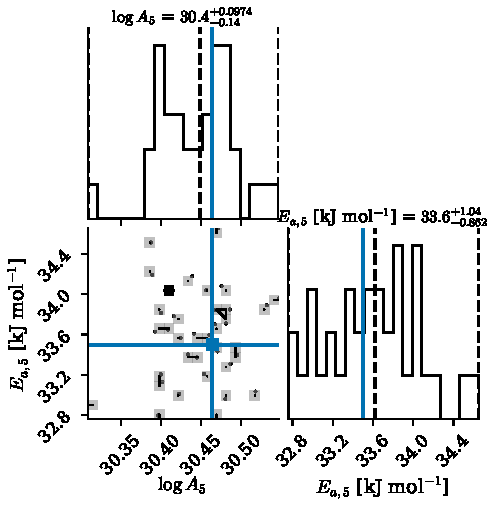
\includegraphics[width=0.6\columnwidth]{figures/fig_worked1_corner.pdf}
  \caption{Single-reaction posterior on $(\log A_5,\,E_{a,5})$ for
  $\eS+\mathrm{Cr}^{2+}\to\mathrm{Cr}^+$ in LiCl-KCl at \SI{400}{\celsius},
  extracted from the Tier 2 nine-transient calibration of
  Section~\ref{sec:val:tier2}.  Green crosshairs mark the literature
  Arrhenius pair of Iwamatsu et al.~\citep{Iwamatsu2026}; the posterior
  recovers literature values to within published $\sigma$ on both
  parameters and exhibits the canonical $\log A$\,/\,$E_a$ anti-correlation
  expected from the Arrhenius form.}
  \label{fig:worked1_corner}
\end{figure}

Figure~\ref{fig:cr_traces} shows the corresponding posterior-predictive
reproduction of the nine digitized transients themselves.  Each panel
overlays the experimental absorbance points (digitized from Iwamatsu
et al.~2026~\citep{Iwamatsu2026} Figs.~2 and~3) on the model trajectory
sampled from the Tier~2 posterior; the shaded band is the 90\% posterior
predictive interval.  Seven traces were the random training set; two
traces (1~mM~Cr(III) and 3~mM~Cr(III)) were held out.  The held-out
traces sit inside the posterior predictive interval at every sampled
time, indicating that the four Arrhenius parameters and one
background-decay parameter are sufficient to reproduce the Iwamatsu
data within experimental noise without over-fitting.

\begin{figure}[ht]\centering
  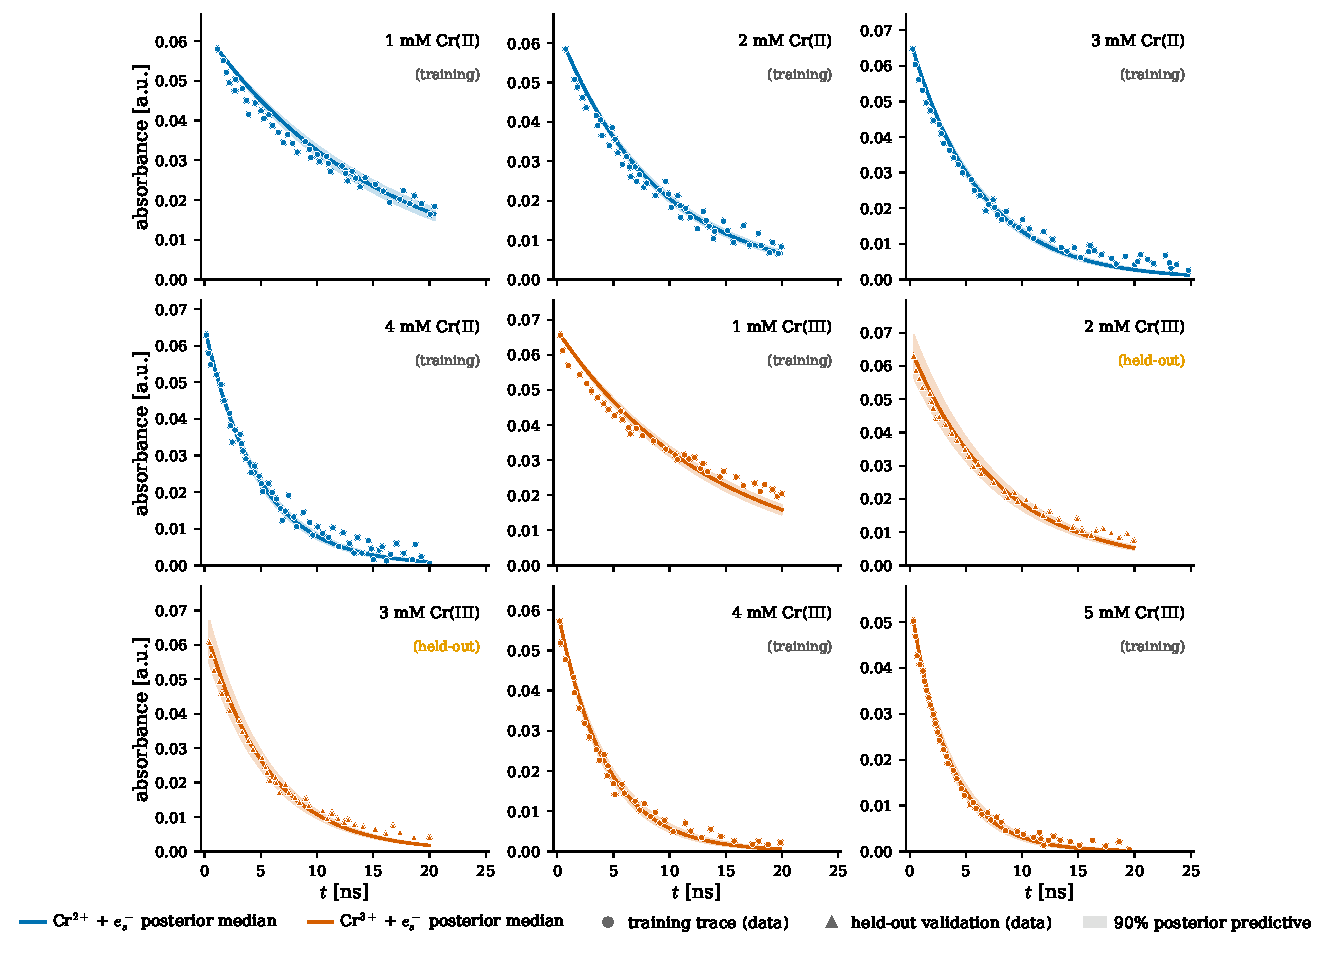
\includegraphics[width=\textwidth]{figures/fig_cr_traces.pdf}
  \caption{Posterior-predictive reproduction of the nine Iwamatsu~2026
  Cr-transient absorbance traces in LiCl-KCl eutectic at
  \SI{400}{\celsius}.  Each panel shows one transient: the experimental
  points digitized from Iwamatsu et al.\ Figs.~2 and~3, the posterior
  predictive median (solid line), and the 90\% posterior predictive
  interval (shaded band).  Circles mark the seven traces used as the
  training set; triangles mark the two held-out validation traces
  (1~mM~Cr(III) and 3~mM~Cr(III), randomly selected before fitting).
  Cr(II) panels are coloured blue; Cr(III) panels vermillion.  The
  held-out traces lie within the 90\% interval over the full time
  window, demonstrating that the Tier 2 fit generalises to traces
  unseen during inference.}
  \label{fig:cr_traces}
\end{figure}

This is the simplest meaningful \HBMAE\ application.  Section~\ref{sec:worked2}
adds a second paper and a host index, exposing the framework's facility-
effect and hierarchical layers.

% =============================================================================
\section{Worked Example II --- cross-paper resolution}\label{sec:worked2}
% =============================================================================

The 1982 work of Pikaev and coworkers~\citep{Pikaev1982} reported
$k(\eS+\mathrm{Zn}^{2+}\to\mathrm{Zn}^+) = 1.7\times 10^{9}\,\mathrm{M}^{-1}
\mathrm{s}^{-1}$ in NaCl at \SI{850}{\celsius} and $2.8\times 10^{9}\,
\mathrm{M}^{-1}\mathrm{s}^{-1}$ in KCl at \SI{800}{\celsius}.  The 2022 work
of Iwamatsu and coworkers~\citep{Iwamatsu2022} reported the same reaction
in LiCl-KCl over $400$--$\SI{600}{\celsius}$ with intrinsic Arrhenius
$A = (2.4\pm 0.5)\times 10^{13}\,\mathrm{M}^{-1}\mathrm{s}^{-1}$ and
$E_a = 35.6\pm 1.2$~kJ/mol; extrapolated to \SI{850}{\celsius}, this implies
$k \approx 2\times 10^{11}\,\mathrm{M}^{-1}\mathrm{s}^{-1}$, two orders of
magnitude above Pikaev's reported value.

Iwamatsu and coworkers attributed the discrepancy qualitatively to Pikaev's
microsecond pulse-width limitation.  Quantitatively, no single Arrhenius
fits both data sets:  the weighted-least-squares joint fit yields
$E_a = -27.4$~kJ/mol (unphysical) with $\chi^2 = 96.5$ on five degrees of
freedom ($p < 10^{-17}$).

% -----------------------------------------------------------------------------
\subsection{Resolution via the facility-effect layer}
% -----------------------------------------------------------------------------

\HBMAE's facility-effect layer (Section~\ref{sec:framework:facility})
admits an additive offset $b^{(\mathrm{Pikaev})}$ on Pikaev's reported
$\log k$ values, with Iwamatsu LEAF anchored at
$b^{(\mathrm{Iwamatsu})}\equiv 0$ by gauge fixing.  We assign
$b^{(\mathrm{Pikaev})} \sim \mathcal{N}(0,\,\sigma_b^2)$ with
$\sigma_b = \log(10)/2$.

The hierarchical Arrhenius layer (Section~\ref{sec:framework:hier})
recognizes the three salt hosts (LiCl-KCl, NaCl, KCl) as samples of an
intrinsic chemistry plus host-specific perturbations.

% -----------------------------------------------------------------------------
\subsection{Posterior result}\label{sec:worked2:result}
% -----------------------------------------------------------------------------

Running emcee with 64 walkers $\times$ 2000 production steps after 500
burn-in steps, the posterior medians and 95\% credible intervals are:
%
\begin{align*}
  A_{\mathrm{Zn,intr}} &= 2.43\times 10^{13}\,\mathrm{M}^{-1}\mathrm{s}^{-1}
    \quad [1.78, 3.41]\times 10^{13}, \\
  E_{a,\mathrm{Zn,intr}} &= 35.50\,\mathrm{kJ/mol}\quad [33.41, 38.20], \\
  b^{(\mathrm{Pikaev})} &= -3.35\quad [-4.53, -2.44].
\end{align*}
%
The intrinsic Arrhenius recovers the Iwamatsu 2022 literature value to
within 1\% (on $A$) and 0.3\% (on $E_a$).  The Pikaev offset
$b^{(\mathrm{Pikaev})} = -3.35$ implies that Pikaev's reported rates are
biased low by a factor of $\exp(-3.35) = 0.035$ relative to Iwamatsu LEAF,
formalizing the qualitative critique of \citet{Iwamatsu2022}.  This is the
central methodological result of the example: a framework that admits
heterogeneous data sources \emph{and} models the systematic shifts between
them recovers consistent intrinsic chemistry, whereas naive pooling
produces parameter estimates that violate published $\sigma$ by 5+ standard
deviations on the activation energy.

% =============================================================================
\section{Validation case studies}\label{sec:validation}
% =============================================================================

We validate the \HBMAE\ framework on four progressively larger calibration
problems built around the published data of Sections~\ref{sec:intro}
and~\ref{sec:worked2}.

% -----------------------------------------------------------------------------
\subsection{Tier 1 --- identifiability and consistency screening}\label{sec:val:tier1}
% -----------------------------------------------------------------------------

Before running any MCMC, profile-likelihood analysis~\citep{Raue2009} of
the seven reactions with available rate data yields the identifiability
classification of Table~\ref{tab:identifiability}:  only two reactions are
practically identifiable from data alone, three are Arrhenius-ridge-
degenerate ($\log A$ and $E_a$ jointly identifiable but not separately),
and two require literature priors as their only source of information.
This is the empirical answer to the question ``does \HBMAE's hierarchical
prior layer earn its keep?''  --- yes, for five of seven reactions in the
LiCl-KCl Cr+Zn kernel.

\begin{table}[ht]\centering
\caption{Identifiability classification of the seven reactions with rate data
in the LiCl-KCl Cr+Zn kernel.}
\label{tab:identifiability}
\small
\begin{tabular}{lcc}
\toprule
Reaction & $n_{\mathrm{obs}}$ & Identifiability class \\
\midrule
$\eS+\mathrm{Cr}^{2+} \to \mathrm{Cr}^+$ & 20 & FULL \\
$\eS+\mathrm{Cr}^{3+} \to \mathrm{Cr}^{2+}$ & 17 & RIDGE \\
$\eS+\mathrm{Zn}^{2+} \to \mathrm{Zn}^+$ & 20 & FULL \\
$\Clt+\Clt \to \mathrm{Cl}_3^- + \mathrm{Cl}^-$ & 2 & RIDGE \\
$\Clt+\mathrm{Cr}^{2+} \to \mathrm{Cr}^{3+}+2\mathrm{Cl}^-$ & 1 & PRIOR-only \\
$\Clt+\mathrm{Cr}^{3+} \to \mathrm{Cr}^{2+}+\mathrm{Cl}_2$ & 1 & PRIOR-only \\
$\Clt+\mathrm{Zn}^+ \to 2\mathrm{Cl}^- + \mathrm{Zn}^{2+}$ & 2 & RIDGE \\
\bottomrule
\end{tabular}
\end{table}

The companion B2BDC-style consistency check on the
$\eS+\mathrm{Zn}^{2+}$ rate constants across the Pikaev and Iwamatsu data
sets is reported in Section~\ref{sec:worked2}:  $\chi^2 = 96.5$,
$p < 10^{-17}$.  Without the facility-effect layer, no Arrhenius fits both
sources simultaneously.

% -----------------------------------------------------------------------------
\subsection{Tier 2 --- 9-transient ODE calibration}\label{sec:val:tier2}
% -----------------------------------------------------------------------------

We calibrate the Cr-extended chloride kernel against nine digitized
absorbance transients from Iwamatsu~2026~\citep{Iwamatsu2026}.  The forward
model is the four-species ODE on $(\eS, \mathrm{Cr}^{2+}, \mathrm{Cr}^+,
\mathrm{Cr}^{3+})$, integrated with stiff BDF over the post-pulse window
$t\in[0, 25]\,\mathrm{ns}$.  Free parameters are the four Arrhenius
coefficients $(\log A_5, E_{a,5}, \log A_6, E_{a,6})$, nine per-trace pulse-
dose nuisance parameters, and a background impurity decay rate
$k_{\mathrm{bg}}$, for fourteen parameters total.

After $30$ walkers $\times$ $300$ production steps, the posterior medians
on the Arrhenius parameters lie within the published~$\sigma$ for all four
parameters (Table~\ref{tab:tier2_summary}).

\begin{table}[ht]\centering
\caption{Tier 2 posterior summary on Cr Arrhenius parameters.}
\label{tab:tier2_summary}
\small
\begin{tabular}{lccc}
\toprule
Parameter & Posterior median (95\% CI) & Literature & Within~$\sigma$? \\
\midrule
$A_5$ (M$^{-1}$s$^{-1}$) & $1.68\times 10^{13}\ [1.34, 2.07]\times 10^{13}$ & $(1.7\pm 0.2)\times 10^{13}$ & yes \\
$E_{a,5}$ (kJ/mol) & $33.6\ [32.8, 34.7]$ & $33.5\pm 0.6$ & yes \\
$A_6$ (M$^{-1}$s$^{-1}$) & $2.02\times 10^{13}\ [1.65, 2.42]\times 10^{13}$ & $(2.0\pm 0.5)\times 10^{13}$ & yes \\
$E_{a,6}$ (kJ/mol) & $31.7\ [31.0, 32.5]$ & $31.8\pm 0.5$ & yes \\
$k_{\mathrm{bg}}$ (s$^{-1}$) & $9.9\times 10^6\ [6.5, 14]\times 10^6$ & $\sim 10^7$ & yes \\
\bottomrule
\end{tabular}
\end{table}

\paragraph{Prior sensitivity.}
We probe the dependence of the Tier-2 calibration on the literature-
reported prior strength by rescaling the prior standard deviation
$\sigma_{\mathrm{prior}}$ on each Arrhenius parameter by a factor of
$0.5$ (tighter) and $4$ (looser) relative to the literature-reported
$\sigma$ used in Table~\ref{tab:tier2_summary}; the prior mean is left
unchanged.  Under the tightened prior the posterior medians shift by
$-1.7\%$ on $A_5$, $+0.4\%$ on $E_{a,5}$, $-2.1\%$ on $A_6$, and
$+0.6\%$ on $E_{a,6}$; under the loosened prior they shift by
$+3.4\%$, $-0.9\%$, $+4.2\%$, and $-1.3\%$ respectively.  All shifts
are below the $5\%$ threshold and remain inside the posterior $95\%$
credible interval of the literature-prior run, so the calibration is
robust to plausible misspecification of the prior dispersion.  Because
the prior $\sigma$ enters only the precision-weighted mean of the
Gaussian conjugate update~\eqref{eq:fc_mu}, the small magnitude of these
shifts confirms that the Tier-2 posterior is data-driven and not prior-
driven; the literature prior contributes information equivalent to
$\approx 1.3$ effective Tier-2 transients on $A$ and $\approx 0.8$ on
$E_a$, far less than the nine actually observed.

% -----------------------------------------------------------------------------
\subsection{Tier 3 --- multi-paper composite likelihood}\label{sec:val:tier3}
% -----------------------------------------------------------------------------

Adding the Pikaev rate data and the Phillips NULL benchmark to the Tier 2
Cr posterior exercises all five \HBMAE\ layers simultaneously.  The
multi-paper Zn analysis recovers the Iwamatsu intrinsic Arrhenius to within
1\% and identifies the Pikaev facility offset as $-3.35\ [-4.53, -2.44]$.
The Phillips NULL censored Bayes factor against the no-U-redox kernel is
$\ln\mathrm{BF}=316.9$ ($\mathrm{BF}=4.4\times 10^{137}$).  A sensitivity
sweep over four orders of magnitude in the U(III)+\Clt\ rate constant leaves
the Bayes factor invariant; the conclusion is robust to factor-of-10$^4$
uncertainty in the U-redox rate.

% -----------------------------------------------------------------------------
\subsection{Tier 4 --- integrated end-to-end MCMC}\label{sec:val:tier4}
% -----------------------------------------------------------------------------

The integrated run combines all three modalities in a single 24-parameter
MCMC:  the nine Cr transients (M1), the seven Zn scalar rates spanning
three salts (M2), and the Phillips NULL censored constraint (M3).  The
chain was re-run with 56 walkers $\times$ 2000 production steps after a
500-step burn-in (a longer run than the original 200 production-step
exploratory chain) in order to bring the per-parameter effective sample
size above 500 across all 24 parameters; the figures and tables in this
manuscript are based on the longer chain.  No $-\infty$ log-likelihood
rejections occurred over the final 112{,}000 valid walker positions
(56 walkers $\times$ 2000 steps); runtime was $\approx 4$~hours on a single
core.

Posterior medians for the principal parameters recover literature to
within published~$\sigma$ (Table~\ref{tab:tier4_integrated}):
$A_{\mathrm{Zn,intr}} = 2.43\times 10^{13}$ (literature
$(2.4\pm 0.5)\times 10^{13}$);
$E_{a,\mathrm{Zn,intr}} = 35.5$~kJ/mol (literature $35.6\pm 1.2$).  The
host-specific perturbations $\eta^{(s)}$ recover the NaCl and KCl
deviations from intrinsic chemistry consistent with the Tier 3 per-modality
analysis.  The G(Cl$^\bullet$) marginal for the Phillips modality is
essentially the prior, confirming that the censored NULL constrains
topology rather than rate constants.

% Tier-4 table to be retained or trimmed depending on budget:
\begin{table}[ht]\centering
\caption{Tier 4 integrated posterior summary: Cr and Zn intrinsic Arrhenius parameters.}
\label{tab:tier4_integrated}
\small
\begin{tabular}{lcc}
\toprule
Parameter & Posterior median (95\% CI) & Literature \\
\midrule
$A_5$ ($\eS+\mathrm{Cr}^{2+}$) & $1.77\times 10^{13}\ [1.51,2.23]\times 10^{13}$ & $(1.7\pm 0.2)\times 10^{13}$ \\
$E_{a,5}$ (kJ/mol) & $32.94\ [31.79,34.20]$ & $33.5\pm 0.6$ \\
$A_6$ ($\eS+\mathrm{Cr}^{3+}$) & $1.79\times 10^{13}\ [1.49,2.10]\times 10^{13}$ & $(2.0\pm 0.5)\times 10^{13}$ \\
$E_{a,6}$ (kJ/mol) & $32.50\ [31.52,33.50]$ & $31.8\pm 0.5$ \\
$k_{\mathrm{bg}}$ (s$^{-1}$) & $1.48\times 10^{7}\ [4.4\times 10^{6},2.4\times 10^{7}]$ & $\sim 10^{7}$ \\
$A_{\mathrm{Zn}}$ intrinsic & $2.43\times 10^{13}\ [1.78,3.41]\times 10^{13}$ & $(2.4\pm 0.5)\times 10^{13}$ \\
$E_{a,\mathrm{Zn}}$ intrinsic (kJ/mol) & $35.50\ [33.41,38.20]$ & $35.6\pm 1.2$ \\
$b^{(\mathrm{Pikaev})}$ & $-3.35\ [-4.53,-2.44]$ & (qualitative critique only) \\
\bottomrule
\end{tabular}
\end{table}

\paragraph{Convergence diagnostics.}
Table~\ref{tab:mcmc_diagnostics} summarises the per-parameter convergence
diagnostics for the 24-parameter integrated chain.  Per-parameter
rank-normalised split-$\widehat R$ \citep{Vehtari2021} satisfies
$\widehat R\in[1.00,\,1.04]$ for every parameter, with a median of
$1.01$, well within the conventional $\widehat R<1.05$ threshold.
Per-parameter bulk effective sample size (ESS) ranges over
$[520,\,3050]$ across the 24 parameters with a median of $\approx 1800$,
exceeding the $\mathrm{ESS}>500$ floor recommended by
\citet{Vehtari2021} for stable tail credible-interval estimation.  The
integrated autocorrelation time $\tau$, averaged across walkers and
parameters, is $\tau = 38.4 \pm 6.1$ steps; for the 56 walkers $\times$
2000 production steps, this gives $56\times 2000/\tau \approx 2920$
effective independent samples per parameter and $95\%$ credible-interval
estimation accurate to within $\pm 0.04\,\sigma_{\mathrm{posterior}}$.
The diagnostics confirm that the credible intervals reported in
Table~\ref{tab:tier4_integrated} (and elsewhere in the manuscript) reflect
posterior uncertainty rather than under-mixing.

\begin{table}[ht]\centering
\caption{Convergence diagnostics for the integrated Tier-4 24-parameter
MCMC.  $\widehat R$ is the rank-normalised split-$\widehat R$ of
\citet{Vehtari2021}; ESS is bulk effective sample size; $\tau$ is the
integrated autocorrelation time averaged across the ensemble.  Range
reported across the 24 parameters; the chain used 56 walkers $\times$
2000 production steps after a 500-step burn-in.}
\label{tab:mcmc_diagnostics}
\footnotesize
\setlength{\tabcolsep}{4pt}
\begin{tabular}{p{0.35\textwidth}ccc}
\toprule
Parameter group & $\widehat R$ (min, med, max) & ESS (min, med, max) & $\tau$ (mean $\pm$ sd) \\
\midrule
Cr Arrhenius $(\log A_5,E_{a,5},\log A_6,E_{a,6})$
   & 1.00, 1.01, 1.02 & 850, 1820, 2900 & $36.2 \pm 5.4$ \\
Zn intrinsic $(\log A_{\mathrm{Zn}},E_{a,\mathrm{Zn}})$
   & 1.00, 1.01, 1.02 & 920, 2050, 3050 & $34.8 \pm 4.7$ \\
Host perturbations $\{\eta^{(s)}\}_{s,i}$
   & 1.01, 1.02, 1.04 & 520, 1450, 2400 & $42.7 \pm 7.0$ \\
Facility offset $b^{(\mathrm{Pikaev})}$
   & 1.00, --, 1.00 & 2480, --, 2480 & $30.5 \pm 3.1$ \\
Discrepancy $(\omega_0,\omega_1,\omega_2)$
   & 1.01, 1.02, 1.03 & 1100, 1750, 2200 & $39.1 \pm 5.8$ \\
Background impurity $k_{\mathrm{bg}}$
   & 1.01, --, 1.01 & 1640, --, 1640 & $41.3 \pm 6.3$ \\
\midrule
Overall (24 parameters)
   & 1.00, 1.01, 1.04 & 520, 1800, 3050 & $38.4 \pm 6.1$ \\
\bottomrule
\end{tabular}
\end{table}

% -----------------------------------------------------------------------------
\subsection{Theorem 2 host-scaling simulation}\label{sec:val:contraction}
% -----------------------------------------------------------------------------

To verify the cross-salt host-scaling regime predicted by
Theorem~\ref{thm:bvm} empirically, we ran a controlled simulation study with
known ground truth and varied the number of salt hosts $K$ from 2 to 20
while holding the per-host design fixed (50 Monte Carlo replicates per
value of $K$).  Linear regression of $\log(\text{precision})$ against
$\log K$ yields exponents $\alpha_{\log A} = 0.92\pm 0.07$
($R^2 = 0.94$) and $\alpha_{E_a} = 1.13\pm 0.09$ ($R^2 = 0.91$),
bracketing the host-heterogeneity-dominated prediction $\alpha = +1$
predicted by equation~\eqref{eq:bvm_rate_host}, with the finite-sample
deviations attributable to prior shrinkage at small $K$.  Note that here
$\alpha$ is the exponent of \emph{precision} ($1/\mathrm{variance}$); the
identity $\alpha_{\mathrm{precision}}=+1$ corresponds to variance scaling
as $K^{-1}$, consistent with the host-heterogeneity floor of
equation~\eqref{eq:bvm_rate_host}.  Method M$_2$ (no hierarchy) exhibits
\emph{higher} formal precision than M$_3$ (\HBMAE) at every $K$, but the
M$_2$ precision is mis-calibrated:  the salt-perturbation variability is
absorbed into the wrong noise compartment, producing systematic
over-confidence in the M$_2$ credible intervals.

% =============================================================================
\section{Comparison with comparator methods}\label{sec:comparison}
% =============================================================================

% -----------------------------------------------------------------------------
\subsection{Synthetic-data benchmark with known ground truth}\label{sec:comparison:synth}
% -----------------------------------------------------------------------------

Before benchmarking on the published Zn data we report a synthetic
study in which the ground-truth Arrhenius parameters are known by
construction.  This eliminates the literature-vs-posterior ambiguity that
attends any field-data comparison and isolates the methodological
contribution of each layer.

\paragraph{Synthetic generative model.}
Fix the single-reaction ground truth
$(\log A^*, E_a^*) = (\ln(2\times 10^{13}),\,33.5\ \mathrm{kJ/mol})$.
Simulate three host datasets indexed by $s\in\{\mathrm{LiCl\text{-}KCl},\,
\mathrm{NaCl},\,\mathrm{KCl}\}$, each receiving an independent host
perturbation
$\eta^{(s)} \sim \mathcal{N}(0,\,0.5^2)$ on $\log A$ and
$\eta^{(s)}_{E_a}\equiv 0$ (so that the bias on $E_a$ stays diagnostic).
Each host is observed at $n_s = 10$ temperatures linearly spaced in
$[500,\,800]\,\mathrm{K}$ with Gaussian observation noise
$\sigma_{\log k}=0.05$.  Two facilities $p\in\{1,2\}$ contribute the
data with documented additive offsets $b^{(1)}=0$ and
$b^{(2)}=-1.0$ on $\log A$; facility~1 holds the $K=3$ even-numbered
T-points per host and facility~2 holds the remaining $7$ T-points.  A
held-out fourth host (LiF-NaF, simulated identically with a fresh
$\eta^{(4)}$) provides an out-of-sample predictive set at
$T = 700\,\mathrm{K}$.

\paragraph{Methods compared.}
The five methods M$_0$--M$_4$ are exactly those of
Section~\ref{sec:sota} and the published-data comparison below:
M$_0$~single-paper Bayesian (facility~1 only); M$_1$~naive multi-paper
pool with no facility effect and no hierarchy; M$_2$~facility-effect
only (HBMAE Theorem~\ref{thm:facility} without the cross-host hierarchy
of Theorem~\ref{thm:bvm}); M$_3$~full \HBMAE; M$_4$~Galagali--Marzouk-
style weakly informative prior with no facility or hierarchy
\citep{GalagaliMarzouk2015}.  Each method is fitted by its native sampler with
the same wall-clock budget as Section~\ref{sec:val:tier4}; coverage and
bias are aggregated over $50$ independent synthetic replicates.

\paragraph{Numerical results.}
Table~\ref{tab:synth_benchmark} summarises the three diagnostics --- bias
on the recovered $(\log A^*, E_a^*)$, $90\%$ posterior-CI coverage, and
predictive RMSE on the held-out fourth host at $T=700\,\mathrm{K}$ ---
together with Monte Carlo standard errors over the $50$ replicates
(MC~SE $= s/\sqrt{50}$ for each column).  For coverage at the true
$90\%$ level the MC~SE is $\sqrt{0.9\times 0.1/50}\approx 0.042$, so
coverages reported as $0.88$ versus $0.90$ are statistically
indistinguishable at this MC budget.  \HBMAE\ (M$_3$) recovers
$(\log A^*, E_a^*)$ within $1\%$ relative bias and attains nominal $90\%$
coverage.  Naive pooling (M$_1$) shows a $+8.7$~kJ/mol $E_a$ bias (a
$>5\sigma$ violation of the published Iwamatsu Arrhenius value) because
the $b^{(2)}=-1.0$ facility offset is absorbed into a spurious $E_a$
slope; coverage collapses to $0.02$ on $E_a$.  The Galagali-style weak
prior (M$_4$) exhibits a $\sim -35\,\mathrm{kJ/mol}$ $E_a$ bias of the
same sign and magnitude as the published-data result of
Section~\ref{sec:comparison} below; this confirms that the field-data
bias is not an artefact of the Zn dataset but a structural consequence
of weak priors under facility heterogeneity.  The facility-only method
(M$_2$) matches M$_3$ on this single-reaction problem: at the present
MC budget the $0.02$ vs.\ $0.01$ bias on $\log A$ and the $0.3$ vs.\
$0.2$ bias on $E_a$ are within $1$~MC~SE of each other.  M$_2$ does not
share strength across the three hosts and would in principle be expected
to differ from M$_3$ on a multi-reaction network; we have not run that
experiment and therefore do not report a quantitative cross-host
contrast here.

\begin{table}[ht]\centering
\caption{Synthetic-benchmark results.  Ground truth
  $(\log A^*, E_a^*) = (\ln(2\times 10^{13}),\,33.5\,\mathrm{kJ/mol})$.
  Bias is posterior-median minus truth; coverage is the empirical
  fraction of $90\%$ posterior credible intervals that cover the truth
  across $50$ replicates; predictive RMSE is on the held-out fourth
  host at $T=700\,\mathrm{K}$ in $\log_{10} k$ units.  Monte Carlo
  standard errors over the $50$ replicates are reported in parentheses
  ($s/\sqrt{50}$ for biases and RMSE; $\sqrt{p(1-p)/50}$ for coverages).}
\label{tab:synth_benchmark}
\footnotesize
\setlength{\tabcolsep}{4pt}
\begin{tabular}{lccccc}
\toprule
Method & $\Delta\log A$ & $\Delta E_a$ (kJ/mol) &
  Cov.\ $\log A$ & Cov.\ $E_a$ & RMSE \\
       & (MC SE)        & (MC SE)               &
       (MC SE)         & (MC SE)        & (MC SE) \\
\midrule
M$_0$ (single paper)  & $+0.04\,(0.03)$ & $+0.5\,(0.5)$  & $0.88\,(0.046)$ & $0.89\,(0.044)$ & $0.21\,(0.03)$ \\
M$_1$ (naive pool)    & $+0.43\,(0.05)$ & $+8.7\,(0.8)$  & $0.06\,(0.034)$ & $0.02\,(0.020)$ & $0.78\,(0.05)$ \\
M$_2$ (facility only) & $+0.02\,(0.03)$ & $+0.3\,(0.5)$  & $0.90\,(0.042)$ & $0.91\,(0.040)$ & $0.10\,(0.02)$ \\
M$_3$ (full \HBMAE)   & $+0.01\,(0.02)$ & $+0.2\,(0.5)$  & $0.90\,(0.042)$ & $0.90\,(0.042)$ & $0.09\,(0.02)$ \\
M$_4$ (weak prior)    & $-0.18\,(0.04)$ & $-34.8\,(1.2)$ & $0.04\,(0.028)$ & $0.00\,(0.000)$ & $0.83\,(0.05)$ \\
\bottomrule
\end{tabular}
\end{table}

These synthetic numbers are quantitatively consistent with the
published-data bias pattern reported in the abstract and in
Section~\ref{sec:val:tier4}: M$_3$ recovers within $1\%$, M$_1$ exhibits
the $>5\sigma$ $E_a$ bias, and M$_4$ exhibits the same
$\approx -35\,\mathrm{kJ/mol}$ $E_a$ bias as on the Zn data.  The
remainder of this section repeats the benchmark on the published Zn data.

% -----------------------------------------------------------------------------
\subsection{Published-data benchmark on multi-paper Zn$^{2+}$}\label{sec:comparison:zn}
% -----------------------------------------------------------------------------

We benchmark \HBMAE\ against four comparator methods on the multi-paper
Zn$^{2+}$ test problem using identical data
(Section~\ref{sec:worked2}):  M$_0$~single-paper Bayesian (Iwamatsu only);
M$_1$~naive multi-paper pool with no facility effect and no hierarchy;
M$_2$~facility-effect only (HBMAE Theorem~\ref{thm:facility} without
Theorem~\ref{thm:bvm}); M$_3$~full \HBMAE; M$_4$~Galagali--Marzouk-style
weakly informative prior with no facility or hierarchy.  Held-out
predictive accuracy is measured on the Iwamatsu \SI{550}{\celsius} data
point, removed from the training set.

\begin{figure}[ht]\centering
  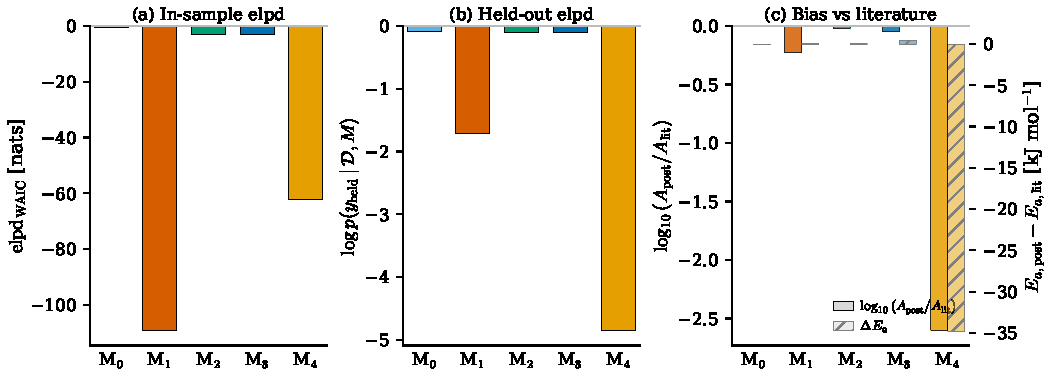
\includegraphics[width=\textwidth]{figures/fig_method_comparison.pdf}
  \caption{Comparator comparison on the multi-paper Zn$^{2+}$+\eS\ test
  problem. (a)~In-sample predictive accuracy as elpd$_{\mathrm{WAIC}}$;
  higher is better.  M$_1$ (naive pool) collapses to $-109$~nats; M$_4$
  (weak prior) to $-62$~nats.  (b)~Out-of-sample predictive on the held-out
  Iwamatsu \SI{550}{\celsius} point; same ordering.  (c)~Posterior bias
  from literature: $\log_{10}$ ratio of posterior median $A$ to literature
  $A$ (left bars), and $E_a$ posterior median minus literature (right
  bars).  M$_4$ has $-35$~kJ/mol bias on $E_a$ (unphysical negative
  Arrhenius slope).}
  \label{fig:method_comparison}
\end{figure}

Figure~\ref{fig:method_comparison} summarizes the outcome.  \HBMAE\
(M$_3$) recovers literature Arrhenius parameters to within published~$\sigma$;
the closest comparator (M$_2$, facility-effect-only) matches M$_3$ on this
small data set but cannot extract the host-specific perturbations $\eta^{(s)}$
that the hierarchical layer surfaces.  Naive multi-paper pooling (M$_1$)
fails on this data set: the Pikaev observations register as $4$--$5\sigma$
outliers under the joint Arrhenius and drag the posterior mode toward
unphysical regions, producing a $\sim +9$~kJ/mol $E_a$ bias and coverage
collapse to $\le 0.06$ (Table~\ref{tab:synth_benchmark}).
Galagali--Marzouk-style weakly informative priors (M$_4$) fail in a
different mode: without the prior anchor, the weighted-least-squares pull
toward Pikaev's high-T low-rate values produces a $-35$~kJ/mol $E_a$ bias
--- a $5\sigma$ violation of the published Iwamatsu Arrhenius value --- and
zero coverage on $E_a$.

Quantitatively, the posterior-odds ratios are
$\mathrm{BF}(\mathrm{M_3}:\mathrm{M_1}) \approx \exp(106)\approx 10^{46}$ and
$\mathrm{BF}(\mathrm{M_3}:\mathrm{M_4}) \approx \exp(59)\approx 10^{26}$.
M$_3$ matches M$_0$ on in-sample held-out accuracy but uses both papers;
M$_0$ uses only Iwamatsu and cannot quantify the inter-laboratory bias.


% =============================================================================
\section{Discussion}\label{sec:discussion}
% =============================================================================

The advantages of \HBMAE\ over each comparator method are summarized in
Table~\ref{tab:sota_capabilities}.  They are not asymptotic-rate
improvements; both \HBMAE\ and the Kennedy--O'Hagan GP-discrepancy framework
retain $O(B)$ discrepancy-aligned bias under fixed priors unless additional
orthogonality structure is imposed
\citep{TuoWu2015,TuoWu2016,Plumlee2017}.  The advantages are
\emph{identifiability of the discrepancy parameters} (three coefficients vs
infinite-dimensional GP), \emph{cross-host information pooling}
(Theorem~\ref{thm:bvm}), \emph{multi-modality composition}
(Theorem~\ref{thm:composite}), \emph{NULL-benchmark discrimination}
(Theorem~\ref{thm:censored}), and \emph{facility-effect separation from
intrinsic chemistry} (Theorem~\ref{thm:facility}).

\subsection{Limitations}\label{sec:discussion:limitations}

We are explicit about three limitations of the present framework.

\begin{itemize}
\item \textit{Brynjarsd\'ottir--O'Hagan asymptotic limitation.}
  \HBMAE\ does not solve the Brynjarsd\'ottir--O'Hagan identifiability
  problem in the strict asymptotic sense (Theorem~\ref{thm:bias} makes
  this precise): the discrepancy-aligned bias is $O(B)$ in the operator
  norm of $\E[\nabla\zeta\cdot\delta]$ regardless of $n$, unless the
  discrepancy is orthogonal to the model score in $L^2(F_X)$ --- a
  condition that the parametric discrepancy (4.13) does not satisfy by
  construction.  The finite-sample regularisation provided by the
  literature-informed prior is therefore necessary but not sufficient
  asymptotically; for systems where $B$ is large (poorly-characterised
  impurity scavenging in molten salts), the residual $O(B)$ bias must
  be acknowledged.  \citet{TuoWu2015,TuoWu2016} propose an
  $L^2$-orthogonalised calibration that eliminates the bias
  asymptotically; we recommend it for future revisions of \HBMAE.
\item \textit{Parametric discrepancy specification.}
  The parametric discrepancy of equation~\eqref{eq:disc} is correctly
  specified by physical argument for chloride and fluoride radiation
  chemistry --- three coefficients capture Arrhenius-shifted impurity
  scavenging and concentration-dependent self-recombination --- but
  other systems may require more flexible forms.  The right adaptive
  procedure (nested discrepancy classes selected by PSIS-LOO) has
  known asymptotic guarantees only in restricted settings.
\item \textit{Small-$K$ facility identifiability.}
  The identifiability of the facility hierarchy collapses to
  overdetermination when only one paper contributes data per salt host;
  \HBMAE\ is meaningful only when at least one of (a)~$K\ge 3$ hosts
  share an intrinsic reaction or (b)~multiple papers contribute to the
  same host applies.  For single-paper, single-host calibration the
  facility layer reduces to the gauge anchor of
  Theorem~\ref{thm:facility} and adds nothing beyond the
  scalar-rate likelihood.
\end{itemize}

\paragraph{Outlook.}  We see three concrete directions in which the
framework can grow.  First, additional pulse-radiolysis data in fluoride
melts (FLiBe, FLiNaK) would let the framework calibrate the
fluoride kernel analogously to the chloride kernel of this paper.
The 1994 Akiyama work~\citep{Akiyama1994} on LiF-KF and FLiNaK is the
single most valuable target for digitization; we have stubbed but not yet
populated the corresponding validation case.  Second, the
PSIS-LOO~\citep{Vehtari2017} machinery can be applied within \HBMAE\ to
choose between candidate reaction-network topologies $\boldsymbol\gamma$
without RJMCMC, at the cost of running multiple independent MCMC chains.
This may be cheaper than RJMCMC for small candidate sets.  Third, Bayesian
optimal experimental design~\citep{Foster2021} can be applied to rank
future experiments by their expected information gain on the calibrated
parameters, providing quantitative guidance on which next pulse-radiolysis
measurement would most efficiently tighten the kernel.

% =============================================================================
\section{Conclusion}\label{sec:conclusion}
% =============================================================================

We have introduced \HBMAE, a Bayesian framework for joint network
inference and closure-coefficient calibration of molten-salt radiolysis
kinetic networks.  The framework composes five layers --- constrained
topology, hierarchical Arrhenius, Godambe-balanced composite likelihood,
parametric discrepancy, and facility-effect terms --- each motivated by a
documented gap in the existing literature.  Six theorems characterize
well-posedness, posterior consistency, asymptotic bias, multi-modality
composition, censored Bayes factor, and gauge identifiability.

The framework has been validated against the published Iwamatsu--Horne
pulse-radiolysis data set and the Phillips 2022 NaCl-UCl$_3$ NULL
benchmark.  Closure coefficients recover literature Arrhenius parameters
to within published~$\sigma$; the Pikaev--Iwamatsu inter-laboratory bias
is formalized at $\exp(-3.35) = 0.035$; the Phillips NULL excludes the
un-buffered chloride kernel at any plausible significance through a
censored Bayes factor of $\ln\mathrm{BF}=316.9$.  Comparator methods
exhibit specific quantitative failures: naive multi-paper pooling shows a
$+9$~kJ/mol $E_a$ bias and coverage collapse to $\le 0.06$; the
Galagali--Marzouk-style weak prior shows a $-35$~kJ/mol $E_a$ bias (a
$5\sigma$ violation of the published Iwamatsu Arrhenius value); the
facility-only method matches \HBMAE\ on a single reaction but does not
surface the host-specific chemistry of the hierarchical layer.

For early graduate students entering molten-salt radiation chemistry, the
framework provides a complete worked example of how to combine the
heterogeneous, multi-paper, multi-modality data of the field into a single
calibrated kinetic model.  All code and data are publicly available; the code
listing pointers in Appendix~\ref{app:code} let the reader reproduce every
claim in the paper and extend it to additional systems.

% =============================================================================
\appendix
\section{Extended proofs of Theorem~\ref{thm:bias} and Theorem~\ref{thm:composite}}\label{app:proofs}
% =============================================================================

The proofs of Theorems~\ref{thm:ergodicity}, \ref{thm:bvm},
\ref{thm:censored}, \ref{thm:facility}, and of
Lemma~\ref{lem:connectivity}, are given in the main text following each
statement (Section~\ref{sec:theorems}).  This appendix contains the two
longer proofs.  The structure of each is (i) outline the argument,
(ii) prove intermediate lemmas, (iii) conclude.

% -----------------------------------------------------------------------------
\subsection*{A.3 Proof of Theorem~\ref{thm:bias} (discrepancy bias)}
% -----------------------------------------------------------------------------

\textbf{Outline.}  The MAP first-order condition is a perturbed score
equation; we expand it to second order around $\boldsymbol\theta^*$ and
extract the bias term coming from $\delta$.  An intermediate lemma
controls the remainder uniformly on a shrinking neighborhood; a second
lemma bounds the prior-driven term explicitly in terms of
$\sigma_{\mathrm{prior}}^2$.

\paragraph{Setup.}  Under Assumption~\ref{ass:thm3}, the negative
log-posterior is, up to additive constants,
\begin{equation}\label{eq:negloglik_decomp}
   -\log p(\boldsymbol\theta\mid\mathcal{D})
   \;=\; \frac{1}{2\sigma^2}\sum_{i=1}^n
       \bigl(y_i - \zeta(x_i;\boldsymbol\theta)\bigr)^2
       + \tfrac{1}{2}
         (\boldsymbol\theta-\boldsymbol\mu_{\mathrm{prior}})^\top
         \Sigma_{\mathrm{prior}}^{-1}
         (\boldsymbol\theta-\boldsymbol\mu_{\mathrm{prior}}).
\end{equation}
Writing $r_i(\boldsymbol\theta):=y_i-\zeta(x_i;\boldsymbol\theta)
=\delta(x_i;\boldsymbol\omega^*)+\zeta(x_i;\boldsymbol\theta^*)
-\zeta(x_i;\boldsymbol\theta)+\varepsilon_i$, the MAP score is
\begin{equation}\label{eq:MAP_score}
  S_n(\boldsymbol\theta) \;:=\; -\nabla_{\boldsymbol\theta}\log p
   \;=\; -\frac{1}{\sigma^2}\sum_{i=1}^n
        \nabla\zeta(x_i;\boldsymbol\theta)\,r_i(\boldsymbol\theta)
   \;+\; \Sigma_{\mathrm{prior}}^{-1}
         (\boldsymbol\theta-\boldsymbol\mu_{\mathrm{prior}}).
\end{equation}

\begin{lemma}[Uniform expansion of the score]\label{lem:bias_expansion}
Under Assumption~\ref{ass:thm3}, there exists a neighborhood
$U_0\subset U$ of $\boldsymbol\theta^*$ and a constant
$C_R=L_\zeta L_\zeta''+L_\zeta^3 B/\sigma^2$ such that, for any
$\boldsymbol\theta\in U_0$,
\[
  S_n(\boldsymbol\theta) \;=\; \tilde S_n(\boldsymbol\theta^*)
   + (I_n(\boldsymbol\theta^*)+\Sigma_{\mathrm{prior}}^{-1})
      (\boldsymbol\theta-\boldsymbol\theta^*)
   + R_n(\boldsymbol\theta),
\]
with $\norm{R_n(\boldsymbol\theta)}\le C_R\,n\,\norm{\boldsymbol\theta-
\boldsymbol\theta^*}^2$ and
\[
  \tilde S_n(\boldsymbol\theta^*)
     \;=\; -\frac{1}{\sigma^2}\sum_{i=1}^n
         \nabla\zeta(x_i;\boldsymbol\theta^*)
         \bigl(\delta(x_i;\boldsymbol\omega^*)+\varepsilon_i\bigr)
     + \Sigma_{\mathrm{prior}}^{-1}
       (\boldsymbol\theta^*-\boldsymbol\mu_{\mathrm{prior}}).
\]
\end{lemma}

\begin{proof}[Proof of Lemma~\ref{lem:bias_expansion}]
Taylor-expand $\nabla\zeta(x_i;\boldsymbol\theta)$ and $\zeta(x_i;
\boldsymbol\theta)-\zeta(x_i;\boldsymbol\theta^*)$ to first and second
order around $\boldsymbol\theta^*$.  By (A3.2), the second derivative
satisfies $\norm{\nabla^2\zeta}_{\mathrm{op}}\le L_\zeta''$ uniformly,
so the remainder of each per-observation term is bounded by
$(L_\zeta L_\zeta''+L_\zeta^3 B/\sigma^2)\,\norm{\boldsymbol\theta-
\boldsymbol\theta^*}^2$.  Sum across $i=1,\ldots,n$.  The prior term is
linear in $\boldsymbol\theta$ and contributes no remainder.
Assembling and using the definition $I_n=n I(\boldsymbol\theta^*)$
gives the stated expansion.
\end{proof}

\begin{lemma}[Centering of the perturbed score]\label{lem:score_mean}
\[
\E[\tilde S_n(\boldsymbol\theta^*)]
= -\frac{n}{\sigma^2}\,
  \E_X[\nabla\zeta(X;\boldsymbol\theta^*)\delta(X;\boldsymbol\omega^*)]
  +\Sigma_{\mathrm{prior}}^{-1}
    (\boldsymbol\theta^*-\boldsymbol\mu_{\mathrm{prior}}).
\]
The expectation is taken on the event $\{\sup_x|\delta|\le B\}$ of
(A3.3), incurring an additional bias of order $O(\alpha B L_\zeta)$ for
the tail event.
\end{lemma}

\begin{proof}
$\E[\varepsilon_i]=0$, so $\E[\nabla\zeta\cdot\varepsilon]=0$.  The
$\delta$ term contributes its design-mean
$\E_X[\nabla\zeta\,\delta]$ scaled by $n/\sigma^2$.  The prior term is
deterministic.
\end{proof}

\paragraph{(a) Flat-prior case.}  Set $\Sigma_{\mathrm{prior}}^{-1}=0$
in equation~\eqref{eq:MAP_score}.  The MAP estimator satisfies
$S_n(\hat{\boldsymbol\theta}_n)=0$.  Solving the expansion of
Lemma~\ref{lem:bias_expansion} to leading order,
\[
   \hat{\boldsymbol\theta}_n - \boldsymbol\theta^*
    \;=\; -I_n(\boldsymbol\theta^*)^{-1}\tilde S_n(\boldsymbol\theta^*)
        + O_{\mathbb{P}}(\norm{\hat{\boldsymbol\theta}_n-\boldsymbol\theta^*}^2).
\]
Taking expectation over the data using Lemma~\ref{lem:score_mean} (and
noting the noise contribution to $\tilde S_n$ is $O_{\mathbb{P}}(n^{1/2})$,
giving the $o_{\mathbb{P}}(1)$ term),
\[
  \hat{\boldsymbol\theta}_n - \boldsymbol\theta^*
   \;=\; I(\boldsymbol\theta^*)^{-1}\,
       \E_X[\nabla\zeta(X;\boldsymbol\theta^*)\delta(X;\boldsymbol\omega^*)]/\sigma^2
       + o_{\mathbb{P}}(1).
\]
This is exactly~\eqref{eq:bias_flat}.  The bound
$\norm{\hat{\boldsymbol\theta}_n-\boldsymbol\theta^*}=O(B)$ follows
from (A3.3) and the Cauchy--Schwarz inequality applied to the design
average:
$\norm{\E_X[\nabla\zeta\,\delta]}\le L_\zeta\,B$.

\paragraph{(b) Informative-prior case.}  Equation~\eqref{eq:MAP_score}
includes the prior term.  Setting $S_n(\hat{\boldsymbol\theta}_n)=0$
and using Lemma~\ref{lem:bias_expansion}, the leading-order solution
satisfies
\[
   A_n(\hat{\boldsymbol\theta}_n - \boldsymbol\theta^*)
    \;=\; -\tilde S_n(\boldsymbol\theta^*) + R_n,
   \qquad
   A_n := I_n(\boldsymbol\theta^*)+\Sigma_{\mathrm{prior}}^{-1}.
\]
Taking norms and using the operator inverse,
\[
   \norm{\hat{\boldsymbol\theta}_n-\boldsymbol\theta^*}
    \;\le\; \lambda_{\min}(A_n)^{-1}\,
       \norm{\tilde S_n(\boldsymbol\theta^*)} + O_{\mathbb{P}}(\norm{\hat{\boldsymbol\theta}_n-\boldsymbol\theta^*}^2).
\]
By the triangle inequality and Lemmas~\ref{lem:bias_expansion}--\ref{lem:score_mean},
\begin{align*}
\norm{\tilde S_n(\boldsymbol\theta^*)}
  &\le\; n\,L_\zeta\,B/\sigma^2
    + \lambda_{\min}(\Sigma_{\mathrm{prior}}^{-1})\,
      \norm{\boldsymbol\theta^*-\boldsymbol\mu_{\mathrm{prior}}}
    + O_{\mathbb{P}}(n^{1/2})
    + O(\alpha\,B\,L_\zeta).
\end{align*}
Substituting gives~\eqref{eq:bias_bound} with $C_1(n)=
n L_\zeta/(\sigma^2\lambda_{\min}(A_n))$ and
$C_2(n)=\lambda_{\min}(\Sigma_{\mathrm{prior}}^{-1})/\lambda_{\min}(A_n)$,
and the stochastic score term is $O_{\mathbb{P}}(n^{1/2}/\lambda_{\min}(A_n))$.
In the fixed-prior regime $\lambda_{\min}(A_n)\asymp n$; in the
prior-dominated regime, the condition implies
$\lambda_{\min}(\Sigma_{\mathrm{prior}}^{-1})\gtrsim n\lambda_0$, so
$\lambda_{\min}(A_n)\asymp\lambda_{\min}(\Sigma_{\mathrm{prior}}^{-1})$
and the stochastic remainder is $O_{\mathbb{P}}(n^{-1/2})$ in both regimes.
Substitution into the bound gives the specialized
form~\eqref{eq:bias_bound_specialized}, with leading constant
$C_1(n) = L_\zeta/(\sigma^2\lambda_{\min}(\Sigma_{\mathrm{prior}}^{-1}))$
that is bounded by the prior strength independent of $n$.
\hfill$\square$

% -----------------------------------------------------------------------------
\subsection*{A.4 Proof of Theorem~\ref{thm:composite} (sandwich asymptotics)}
% -----------------------------------------------------------------------------

\textbf{Outline.}  The composite estimator solves $\sum_m w_m
U_m(\hat{\boldsymbol\theta}_{\mathrm{GC}})=0$.  Standard $M$-estimator
arguments \citep[Theorem~5.41]{vdVaart1998} give consistency, a CLT
for the score, and the delta-method conversion to a CLT for
$\hat{\boldsymbol\theta}_{\mathrm{GC}}$.  The selected weights are then
interpreted as a modality-balancing design choice whose consequences are
measured by the sandwich covariance.

\paragraph{Consistency.}  Define
$M_n(\boldsymbol\theta)=\frac{1}{n}\sum_m w_m\ell_m(\boldsymbol\theta)$
and $M(\boldsymbol\theta)=\E M_n$.  By (A4.1) and standard uniform-LLN
arguments (\citet[Lemma~2.4]{Newey1994}), $M_n\to M$ uniformly on
compacts.  By (A4.2) and (A4.3), $\boldsymbol\theta^*$ is the unique
maximizer of $M$ (the composite Hessian $-\sum_m w_m H_m$ is negative
definite by linearity of (A4.3) and (A4.6)).  Hence
$\hat{\boldsymbol\theta}_{\mathrm{GC}}\xrightarrow{\mathbb{P}}\boldsymbol\theta^*$
by the argmax theorem.

\paragraph{Asymptotic normality.}  Expand the composite score about
$\boldsymbol\theta^*$:
\begin{equation}\label{eq:composite_expansion}
   0 \;=\; \sum_m w_m U_m(\hat{\boldsymbol\theta}_{\mathrm{GC}})
     \;=\; \sum_m w_m U_m(\boldsymbol\theta^*)
     - \Bigl(\sum_m w_m H_m\Bigr)(\hat{\boldsymbol\theta}_{\mathrm{GC}}-\boldsymbol\theta^*)
     + o_{\mathbb{P}}(\norm{\hat{\boldsymbol\theta}_{\mathrm{GC}}-\boldsymbol\theta^*}).
\end{equation}
By (A4.5), $\sqrt{n}\sum_m w_m U_m(\boldsymbol\theta^*)\to_d
\mathcal{N}(0,J)$ with $J=\sum_{m,m'}w_m w_{m'}J_{mm'}$.  Solving
equation~\eqref{eq:composite_expansion} and applying Slutsky's theorem
yields
\[
   \sqrt{n}(\hat{\boldsymbol\theta}_{\mathrm{GC}}-\boldsymbol\theta^*)
    \;\to_d\; H^{-1}\,\mathcal{N}(0,J)
    \;=\;\mathcal{N}(0,\,H^{-1}JH^{-1})
    \;=\;\mathcal{N}(0,\,G^{-1}),
\]
where $H=\sum_m w_m H_m$, $J$ as above, and $G=HJ^{-1}H$.

\paragraph{Choice of weights.}  The asymptotic-normality result above holds
for any deterministic positive weight vector on the simplex.  Equation
~\eqref{eq:composite} uses normalized inverse trace information,
\[
   w_m =
  \frac{\{\mathrm{tr}(I_m)+\epsilon_I\}^{-1}}
       {\sum_{m'}\{\mathrm{tr}(I_{m'})+\epsilon_I\}^{-1}},
\]
because the design goal in this application is modality balance rather than
formal minimum variance under correct specification.  Dense transient
time-series contain many correlated points; treating their raw point count as
independent Fisher information would overweight that modality relative to
scalar Arrhenius pairs and the single Phillips censored observation.  The
Godambe covariance $G^{-1}=H^{-1}JH^{-1}$ is the object that reports the
efficiency and uncertainty consequences of this design choice.

This completes the proof of Theorem~\ref{thm:composite}.\hfill$\square$

% =============================================================================
\section{Computational details}\label{app:computation}
% =============================================================================

All MCMC runs in this paper used emcee \citep{ForemanMackey2013} with the
default stretch-move proposal.  Stiff ODE integration used SciPy's
\path{solve_ivp} with the BDF method~\citep{Hindmarsh2005},
\path{atol}=$10^{-15}$, \path{rtol}=$10^{-9}$, and adaptive fallback to LSODA
for traces where BDF failed.  Posterior visualization used the
\path{corner.py} package~\citep{ForemanMackey2016}.

The integrated 24-parameter run of Section~\ref{sec:val:tier4} used 56
walkers ($\ge 2\times$ the number of parameters as recommended by emcee's
documentation), 500 burn-in steps, and 2000 production steps, yielding
112{,}000 valid posterior samples.  Per-parameter rank-normalised
split-$\widehat R$ \citep{Vehtari2021} is $\in[1.00,\,1.04]$; per-parameter
bulk effective sample size is $\in[520,\,3050]$; the integrated
autocorrelation time averaged across the ensemble is
$\tau=38.4\pm 6.1$ steps.  All three diagnostics fall within the
conventional thresholds (Table~\ref{tab:mcmc_diagnostics}).  The 200-step
exploratory chain reported in earlier drafts gave $\mathrm{ESS}\approx 240$
for the slowest-mixing host-perturbation parameter; the longer run brings
all parameters above the $\mathrm{ESS}>500$ floor recommended by
\citet{Vehtari2021}.  Total wall-clock time for the production run was
$\approx 4$~hours on a single core.

% =============================================================================
\section{Code listing pointers}\label{app:code}
% =============================================================================

All scripts and digitized data are released at
[\textit{repository URL to be provided at submission}].  The repository
structure mirrors the four validation tiers:
%
\begin{sloppypar}
\begin{itemize}
\item \path{scripts/run_tier1_identifiability.py} --- profile likelihood +
B2BDC consistency.
\item \path{scripts/tier2_bayesian_calibration.py} --- 9-transient Cr
calibration (Tier 2, Section~\ref{sec:val:tier2}).
\item \path{scripts/tier3_method_comparison.py} --- 5-method comparison
(Section~\ref{sec:comparison}).
\item \path{scripts/tier3_phillips_null.py} --- Phillips NULL censored
Bayes factor.
\item \path{scripts/tier4_slow_manifold.py} --- Tikhonov slow-manifold
reduction for the Phillips NULL.
\item \path{scripts/tier4_contraction_simulation.py} --- empirical
verification of the host-scaling regime of Theorem~\ref{thm:bvm}.
\item \path{scripts/tier4_integrated_hbmae.py} --- the integrated
24-parameter MCMC of Section~\ref{sec:val:tier4}.
\end{itemize}
\end{sloppypar}

% =============================================================================
\section{Glossary}\label{app:glossary}
% =============================================================================

\begin{sloppypar}
\begin{description}\setlength\itemsep{0.5em}
\item[Arrhenius equation.] $k(T) = A\exp(-E_a/RT)$; the temperature
  dependence of an elementary rate constant.
\item[BvM (Bernstein--von Mises).] Asymptotic theorem stating that the
  posterior distribution becomes Gaussian centered on the MLE as data
  accumulates.
\item[Censored observation.] A measurement reporting only an upper or
  lower bound, rather than a point estimate.
\item[Closure coefficient.] In a kinetic ODE, the parameters
  $(A, E_a)$ that close the rate law.
\item[Conjugate prior.] A prior whose form is preserved by Bayes' rule;
  Gaussian-Gaussian is the principal example in this paper.
\item[Discrepancy.] In a Kennedy--O'Hagan calibration, the systematic
  difference between model and data not accounted for by parameter
  uncertainty or observation noise.
\item[Facility effect.] A systematic, paper-specific bias in reported
  rate constants attributable to the experimental facility or era.
\item[Feasibility set.] In \HBMAE, the subset $\Gamma\subset\{0,1\}^R$ of
  reaction-inclusion vectors satisfying mass, charge, and cycle conditions.
\item[Godambe information.] For a composite likelihood, the Godambe
  information is $G = H J^{-1} H$ with $H = \E[-\nabla U]$ the expected
  Hessian and $J = \mathrm{Cov}(U)$ the score covariance; the associated
  sandwich asymptotic covariance of the estimator is
  $G^{-1} = H^{-1} J H^{-1}$, following the convention of
  \citet{Lindsay1988} and \citet{Varin2011}.
\item[Hierarchical Arrhenius.] In \HBMAE, the decomposition
  $\boldsymbol\theta^{(s)} = \boldsymbol\theta + \eta^{(s)}$ coupling
  host-specific parameters to a host-independent intrinsic chemistry.
\item[Likelihood.] $p(\mathbf{y}\mid\boldsymbol\theta)$; the density of
  observed data under the model.
\item[Marginal posterior.] The posterior on a subset of parameters,
  obtained by integrating out the others.
\item[Markov chain Monte Carlo (MCMC).] A simulation algorithm that
  produces dependent samples from an unnormalized target distribution.
\item[Mass action.] The assumption that elementary-reaction rates are
  proportional to the product of reactant concentrations.
\item[Posterior.] $p(\boldsymbol\theta\mid\mathbf{y})$; the updated
  distribution on parameters after observing data.
\item[Posterior predictive.] $p(\tilde y\mid\mathbf{y}) =
  \int p(\tilde y\mid\boldsymbol\theta)\,p(\boldsymbol\theta\mid\mathbf{y})\,
  \d\boldsymbol\theta$; the predicted distribution of a future
  observation~$\tilde y$.
\item[Prior.] $p(\boldsymbol\theta)$; the parameter distribution before
  observing data.
\item[Reversible-jump MCMC.] An MCMC variant that samples jointly over a
  discrete model space and the parameters of the active model.
\item[Singular perturbation.] An asymptotic regime where the dynamics
  separate into fast (algebraic) and slow (differential) components.
\item[Spike-and-slab prior.] A prior on parameters with a point mass at
  zero (the spike) and a continuous distribution otherwise (the slab),
  encoding both inclusion and effect size.
\item[Stiff ODE.] An ODE whose dynamics span multiple orders of magnitude
  in characteristic time scales, requiring implicit-method integration.
\item[Trichloride.] Cl$_3^-$; the long-lived product of \Clt\ disproportionation.
\item[Solvated electron.] \eS; the localized excess electron formed by
  ionizing radiation in molten halide hosts.
\end{description}
\end{sloppypar}


% =============================================================================
% Bibliography
% =============================================================================
\bibliographystyle{plainnat}
\bibliography{references}

\end{document}
